%----------------------------------------------------------------------------------------
%	MASTERS REPORT LAYOUT AND PACKAGES
%----------------------------------------------------------------------------------------

\documentclass[twoside,twocolumn]{article}
\raggedbottom
\usepackage{blindtext}
\usepackage{hyperref}
\usepackage[sc]{mathpazo}
\usepackage[T1]{fontenc}
\linespread{1.05}
\usepackage{microtype}
\usepackage{amsmath}
\usepackage{amssymb}
\usepackage{graphicx}
\usepackage{tabulary}
\usepackage{mathtools}
\usepackage[english]{babel}
\usepackage[T1]{fontenc}
\usepackage[hmarginratio=1:1,top=32mm,columnsep=25pt]{geometry}
\usepackage[hang, small,labelfont=bf,up,textfont=it,up]{caption}
\usepackage{booktabs}
\usepackage{lettrine}
\usepackage{enumitem}
\setlist[itemize]{noitemsep}
\usepackage{abstract}
\renewcommand{\abstractnamefont}{\large\scshape}
\renewcommand{\abstracttextfont}{\normalfont\small\itshape}
\DeclareRobustCommand{\pc}{\genfrac(){0pt}{}}
\usepackage{titlesec}
\titleformat{\section}[block]{\large\scshape}{\thesection.}{1em}{}
\font\subsecfont = cmr12 at 11pt
\titleformat{\subsection}[block]{\subsecfont\scshape}{\thesubsection.}{1em}{}
\usepackage{fancyhdr}
\pagestyle{fancy}
\fancyhead{}
\fancyfoot{}
\fancyhead[C]{Source Detection and Localization through Materials $\bullet$ Final Report $\bullet$ May 2019}
\fancyfoot[RO,LE]{\thepage}
\usepackage{titling}
\usepackage{hyperref}
\usepackage{subcaption}

%----------------------------------------------------------------------------------------
%	TITLE SECTION
%----------------------------------------------------------------------------------------

\setlength{\droptitle}{-4\baselineskip}
\pretitle{\begin{center}\Huge\bfseries}
\posttitle{\end{center}}
\font\myfont=cmr12 at 20pt
\title{\myfont Modeling Gamma Source Detection and Localization through Materials}
\author{
\textsc{Darrell Stepter} \\
\normalsize {University of California, Berkeley} \\
\normalsize {darrell.stepter@berkeley.edu} \\
%\normalsize {\today}
}

\renewcommand{\maketitlehookd}{%
\begin{abstract}
\label{sec:abs}
The ability to detect and localize radioactive sources in an urban environment is critical to national security. A wide-range of detection systems have demonstrated the ability to detect the presence of radioactive materials through walls and localize by producing images of the comparative gamma flux. Localization is merely visually locating the "hot spot" in the image, which can be greatly effected by gamma scattering in walls. This inaccurate localization requires search and recovery personnel to conduct a broader search, increasing their exposure time and accumulated dose, instead of moving directly to the material of interest. Additionally, the extended search duration provides hostile actors time to move, detonate, or take any other action to impede recovery operations. The ability to quantify (i.e. determine the exact flux and energy) the flux through building surfaces could allow search and recovery personnel to externally detect, identify (by energy), and localize (by focusing on the target energy) sources. This paper examines how quantification can provide highly accurate source localization through materials. Specifically, a model was developed that would produce a quantified surface flux from a source within a building. With the quantified surface flux simple image processing techniques were applied to provide highly accurate source localization.

\end{abstract}
}

%----------------------------------------------------------------------------------------

\begin{document}
\maketitle

%----------------------------------------------------------------------------------------
%	ARTICLE CONTENTS
%----------------------------------------------------------------------------------------

\section{Introduction}
\label{sec:intro}
\noindent Unauthorized acts involving the use of radiological material, particularly in urban environments, is of national concern. The effects of a dirty bomb or radiological dispersal device being detonated in a densely-populated area would be catastrophic from a health, financial, and psychological standpoint. The ability of radiological search and recovery personnel to quickly to detect, localize and recover radioactive sources is critical for reducing this threat.
\\\\
The military normally breaks search and recovery down in to four operational areas:
\begin{itemize}
  \item Beyond Line of Sight (BLOS) - satellite and high altitude reconnaissance systems
  \item Far Area - fast moving airborne systems
  \item Near Area - ground vehicle, helicopter, and Unmanned Aerial Systems (UAS)
  \item Objective Area - Unmanned Ground Systems (UGS) and dismounted personnel
\end{itemize}
BLOS and Far Area operations are normally conducted by the Air Force while Near and Objective Area operations are conducted by Army and Marine Corps Technical forces or Special Operations Forces, depending on the threat, location, and operational availability of forces. Advances in UAS mounted detection has allowed for the collection of information in the Near Area that once could only be collected in the Objective Area. These advances and additional ones in UGS will minimize personnel exposure in the Objective Area. The goal of this work is to simulate a search and recovery scenario to explore the potential benefits of surface flux quantification. Specifically, to develop a quick and accurate localization method to minimize the exposure time of search and recovery personnel.

\subsection{Motivation}
\noindent In the early spring of 2018 the Defense Threat Reduction Agency (DTRA) invited numerous Universities, National Labs, and Commercial companies to partake in an Unmanned Search Technology Demonstration at Camp Roberts, CA. DTRA personnel placed an unknown source, of unknown activity, in a small village and participants were to detect and localize the source. Lawrence Berkeley National Laboratory (LBNL) demonstrated its Localization and Mapping Platform (LAMP).

\begin{figure}[!htb]
  \centering
  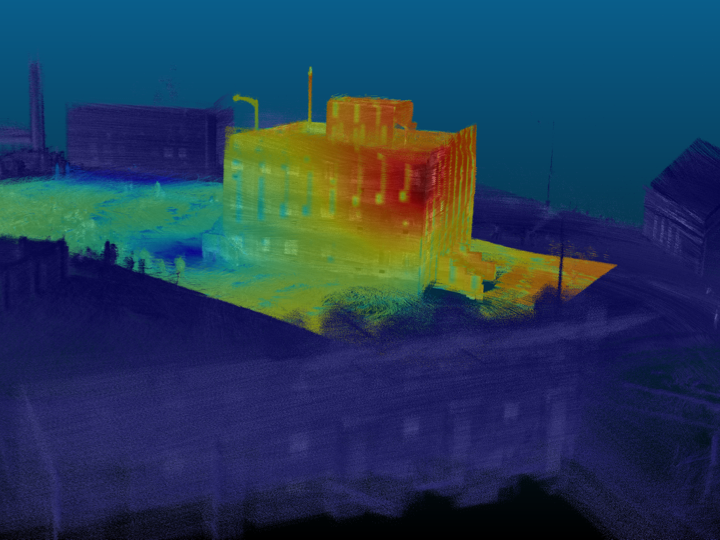
\includegraphics[width=\columnwidth]{images/Heatmap}
  \caption{Gamma "Heatmap" produced by LAMP at DTRA Unmanned Search Technology Demonstration}
  \label{fig:Heatmap}
\end{figure}

Fig. \ref{fig:Heatmap} displays the "Heatmap" produced by LAMP. While it is clear that the source is located near the corner of the building, which floor it is on is unclear. Furthermore, the source and its activity are still unknown. That information could drastically alter the methods used by recovery personnel. Quantification would allow for source identification by energy, activity calculation by flux, and precise localization filtering scattered gammas (filter by peak energy).
\\\\
The remainder of the paper describes methods for achieving this objective. Section \ref{sec:Model} details the development of the model and the tools used to conduct the simulations.  Section \ref{sec:Methodology} discusses how quantification and localization are simulated. Section \ref{sec:results} describes the results of the quantification and localization simulations. Finally, Section \ref{sec:conclusion} describes the limitations of this study and provides recommendations for future work.


\section{Model}
\label{sec:Model}
\subsection{Modeling Tools}
\noindent The main tool used for this project is the Medium-Energy Gamma-ray Astronomy library (MEGAlib). MEGAlib is a set of software tools which are designed to simulate and analyze data of gamma-ray detectors, with a specialization on Compton telescopes. While MEGAlib was originally developed for astrophysics, it has been expanded and used for ground based applications such as medical imaging and environmental monitoring. MEGAlib contains a geometry and detector description tool for the detailed modeling of different detector types and characteristics, and provides an easy to use simulation program based on Geant4. Within MEGAlib, the two tools used to simulate the search scenario are Geometry for MEGAlib (Geomega) and the Cosmic Simulator (Cosima). Geomega allows for the creation of precise and unique geometries in which to run simulations \cite{cosima}. Cosima generates particles within the Geomega geometry and provides detailed information on every particle interaction in an output sim file \cite{cosima}. Of interest to this project, the Cosima output provides positional information on the particles interaction in material (scattering) and where it impacted the detector.

\begin{figure}[!htb]
  \centering
  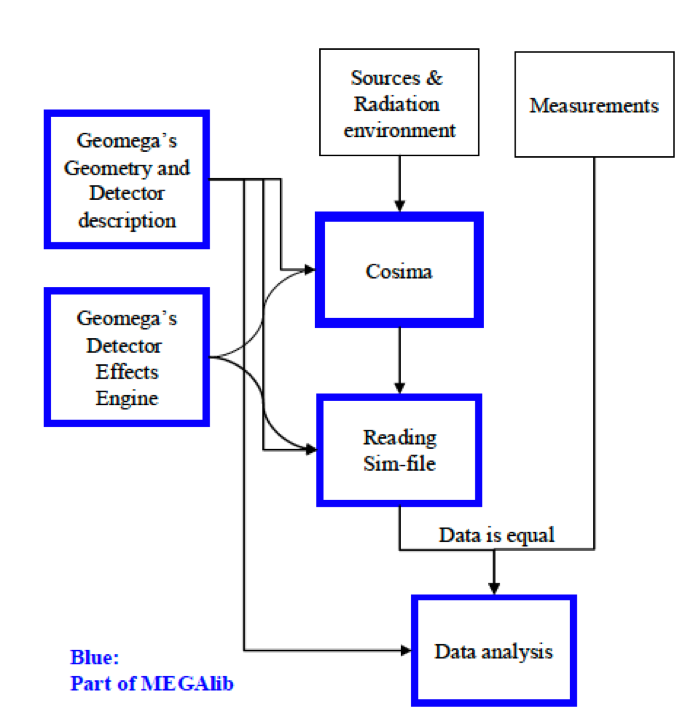
\includegraphics[width=\columnwidth]{images/MEGAlib}
  \caption{Work flow of MEGAlib simulation}
  \label{fig:MEGAlib}
\end{figure}

Fig. \ref{fig:MEGAlib} displays the work flow of a MEGAlib simulation. In addition to MEGAlib, extensive python coding is required to parse the sim file, quantify surface flux, and localize sources.

\subsection{Simulating Camp Roberts}
The intended model is a detector system mounted on a UAS conducting a flight around a target building. In addition to unknown source, activity, and location, the geometry and material composition of the buildings at Camp Roberts are also unknown. Moreover, distance and lack of access made measuring and material sampling an unfeasible option. Instead, a standard three story concreter building on an asphalt slab was modeled using ASTM Building and Construction Standards. Material composition of concrete and asphalt were modeled using the Pacific Northwest National Laboratory Compendium of Material Composition for Radiation Transport Modeling \cite{compendium}. Tables \ref{table:concrete} and \ref{table:asphalt} show the material composition of concrete and asphalt.

\begin{table}[!htp]
 \caption{Material Composition of Concrete}
  \begin{center}
    \begin{tabulary}{\columnwidth}{ccc}
      \hline
      Concrete & 2.3 g/cm$^{3}$\\ \hline
      Element & Weight Fraction\\ \hline
      H & 0.022100  \\
      C & 0.002484 \\
      O & 0.574930 \\
      Na & 0.015208 \\
      Mg & 0.001266 \\
      Al & 0.019953 \\
      Si & 0.304627 \\
      K & 0.010045 \\
      Ca & 0.042951 \\
      Fe & 0.006435 \\ \hline
    \end{tabulary}
  \end{center}
  \label{table:concrete}
\end{table}

\begin{table}[!htp]
 \caption{Material Composition of Asphalt Pavement}
  \begin{center}
    \begin{tabulary}{\columnwidth}{ccc}
      \hline
      Asphalt & 2.5784 g/cm$^{3}$\\ \hline
      Element & Weight Fraction\\ \hline
      H & 0.007781\\
      C & 0.076175\\
      N & 0.000363\\
      O & 0.459103\\
      Na & 0.011659\\
      Mg & 0.021757\\
      Al & 0.051009\\
      Si & 0.231474\\
      S & 0.002804\\
      K & 0.017058\\
      Ca & 0.084471\\
      Ti & 0.003403\\
      V & 0.000024\\
      Mn & 0.000362\\
      Fe & 0.031375\\
      Ni & 0.000002\\
      Pb & 0.001179\\ \hline
    \end{tabulary}
  \end{center}
  \label{table:asphalt}
\end{table}

To ensure the model provided multiple use cases, the first floor was modeled with an open door, the second floor was partitioned into four equally sized rooms, and the top floor was fully enclosed. The exact measurement of the building are 6.2m x 6.2m x 9m, with a wall, roof, and floor thickness of 10 cm. The asphalt slab is 20m x 20m x 0.5m. The flight path of the detector around the building is approximated using a cylindrical blackbody absorber (i.e. every simulated particle will be collected) with a cap around the building. The blackbody absorber has a 10m radius centered on the building and is 14m tall.

\begin{figure}[!htb]
  \centering
  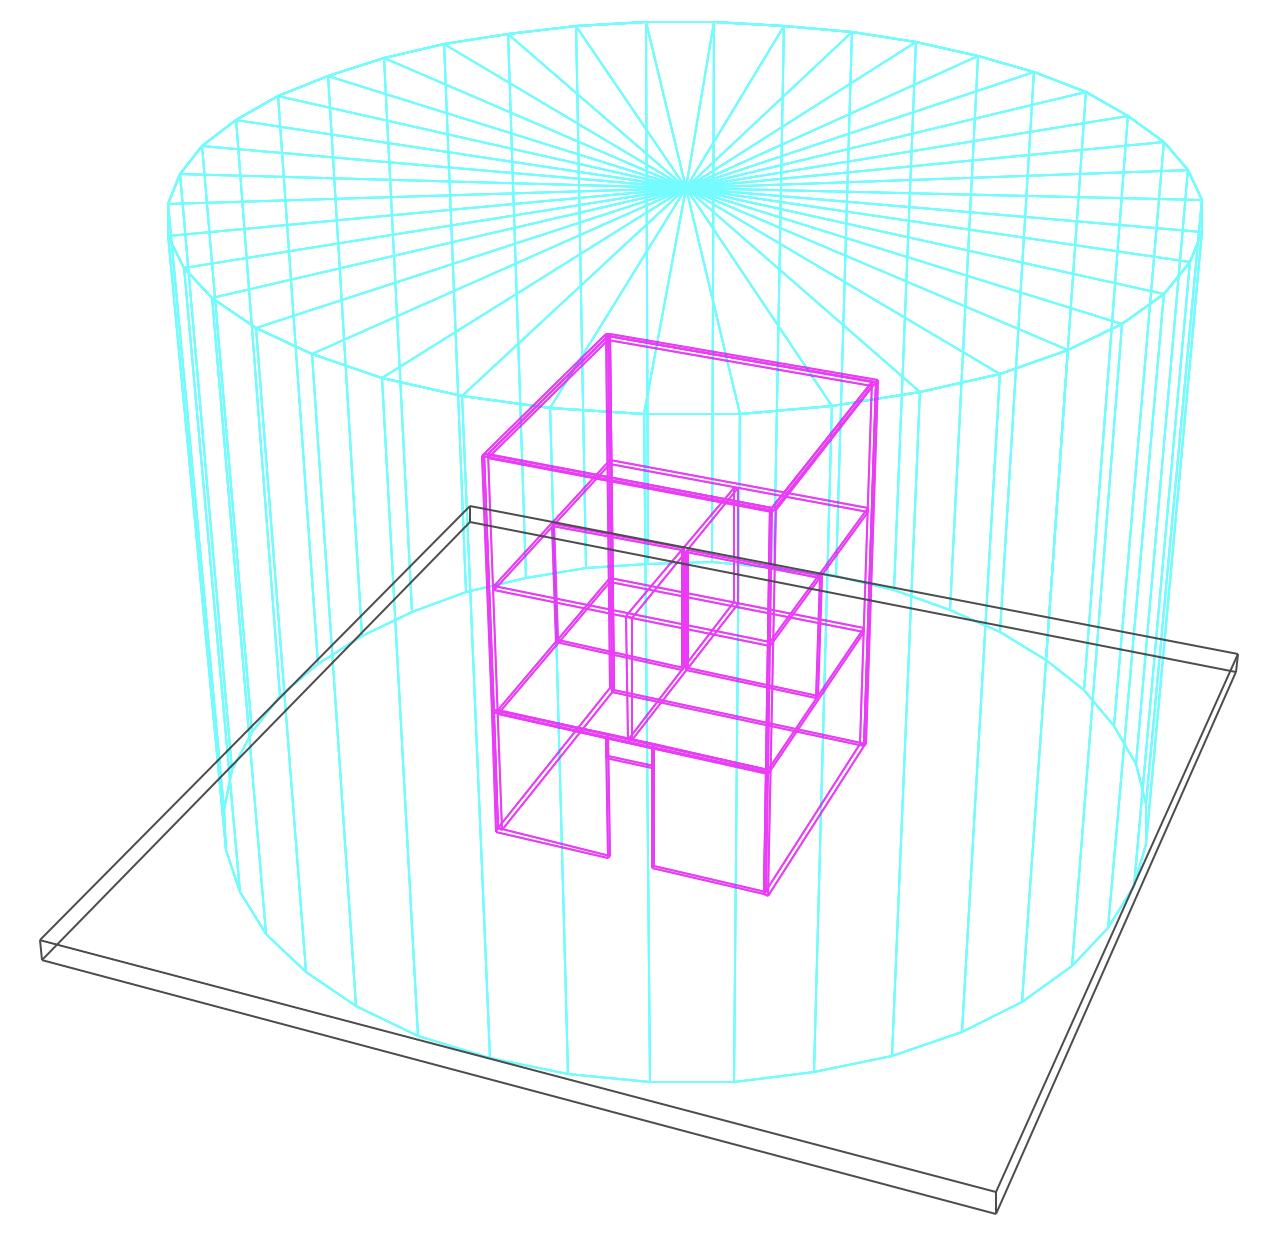
\includegraphics[width=\columnwidth]{images/model}
  \caption{Geomega model of building (pink), slab (black), and detector (cyan)}
  \label{fig:model}
\end{figure}

Fig. \ref{fig:model} displays the simulation geometry. The source was simulated in nine locations (three on each floor) of varying height and distance from detector.

\begin{table}[!htp]
 \caption{Source Locations for Simulations}
  \begin{center}
    \begin{tabulary}{\columnwidth}{ccccc}
      \hline
      Floor & Location & x [cm] & y [cm] & z [cm] \\ \hline
      1 & Central & 50 & -50 & 50 \\
      1 & Middle & 150 & -150 & 150 \\
      1 & Wall & 250 & -250 & 250 \\
      2 & Central & 50 & -50 & 350 \\
      2 & Middle & 150 & -150 & 450 \\
      2 & Wall &250 & -250 & 550 \\
      3 & Central & 50 & -50 & 650 \\
      3 & Middle & 150 & -150 & 750 \\
      3 & Wall & 250 & -250 & 850 \\ \hline
    \end{tabulary}
  \end{center}
  \label{table:positions}
\end{table}

Table \ref{table:positions} shows the simulated source locations. The floor at the center of the building is at (0,0,0).

\subsection{The Inverse Square Law of Radiation}
\label{subsec:inverse}
\noindent The counts registered by a detector is governed by Poisson statistics and decreases inversely with the square of distance. Assuming the source emits radiation isotropically, the count rate in the detector, CR, in s$^{-1}$ can be defined as \cite{morse}:

\begin{align}
CR = \frac{A B A_{d} \eta} {4\pi r^2} \label{eq1}
\end{align}

Where $A$ is the source activity, $B$ is the branching ratio, $A_{d}$ is is the detector area, $\eta$ is the detector efficiency, and $r$ is the distance from the source to the detector. When gammas are transmitted through materials the possibility on interaction with materials is governed by the density of the material, $\rho$, the mass attenuation coefficient for that specific energy, $\mu$/$\rho$, and the attenuation length, $\Delta$$L$.The count rate of full energy deposition in to detector can be defined as \cite{morse}:

\begin{align}
CR = \frac{A B A_{d} \eta e^(\frac{\mu}{\rho}\Delta L)} {4\pi r^2} \label{eq2}
\end{align}
\\\\
Based on the above principle, the detector response in simulations should be highly dependent on the distance of the source from the detector and the amount of attenuation.


\section{Methodology}
\label{sec:Methodology}
\subsection{Simulating Quantification}
\noindent A method for quantification on a mobile detection platform has yet to be achieved. However, through simulation, a quantified flux can be derived and the benefits of quantification can be thoroughly explored. The steps to produce a quantified surface flux are as follows:

\begin{enumerate}
	\item Run Simulation
	\item Parse simulation output for interactions of interest (detector hits)
	\item Back-project detector hit to last interaction in material (scattered) or to source (full transmission)
  \item Determine where particles exited building surface
  \item Subdivide surface to produce quantified surface flux
\end{enumerate}

\subsection{Localization}
\noindent Because gammas are generated isotropically when they hit a plane they will produce a circular "hot spot." The point on the plane normal to the source will see the greatest transmission and transmission will reduce radially as the attenuation length increases with the reduction in incident angle. For this reason a circular fit is used to localize the source. The steps to localize are as follows:

\begin{enumerate}
	\item Implement Canny Edge Finding Algorithm on each wall\cite{canny}
  \begin{enumerate}
  	\item Apply Gaussian filter to smooth the image in order to remove the noise
  	\item Find the intensity gradients of the image
  	\item Thin edges to 1-pixel be removing non-maximum pixels of the gradient
    \item Suppress weak edges
  \end{enumerate}
	\item Conduct Random Sample Consensus (RANSAC) fit to circular model to each wall\cite{ransac}
  \begin{enumerate}
  	\item Select a random subset of the original data (hypothetical inliers)
  	\item Fit circular circular model to hypothetical inliers
  	\item Test remaining data to circular model
    \item Those points that fit the estimated model well are considered as part of the consensus set
    \item Re-estimate model using all members of the consensus set
    \item The center of the circular model is the estimated source location on that plane
  \end{enumerate}
  \item Calculate line segments connecting estimated source location for East/West and North/South planes
  \item Estimated source location is line intersection or midpoint of shortest distance between lines
\end{enumerate}

\subsection{Hypothesis}
\noindent
It hypothesized that gating on full source energy will produce a smaller hot spot on which to localize and therefore will provide a more accurate source location than total counts. Additionally, the simulations closest to the walls would exhibit less radial dispersal than simulations closer to the center of the building and therefore will provide more accurate source locations.


\section{Results}
\label{sec:results}
\noindent Each simulation generated six million 1332.492 keV gammas, indicative of a $^{60}$Co source.

\subsection{Quantification}
\noindent The following results are from the source located on the first floor in the central position as described in Table \ref{table:positions}.

\begin{figure}[!htb]
  \centering
  \includegraphics[width=\columnwidth]{images/5Det_Comparison_1fl_cen}
  \caption{Flux incident on detector plane}
  \label{fig:DetFlux1C}
\end{figure}

Fig. \ref{fig:DetFlux1C} shows the flux incident on the detector plane around the building. The flux is quantified into gross counts, full energy, partial energy, and scattering from the ground. There is a large amount of full energy depositions because the source location provides a clear line of sight to the detector.

\begin{figure}[!htb]
  \centering
  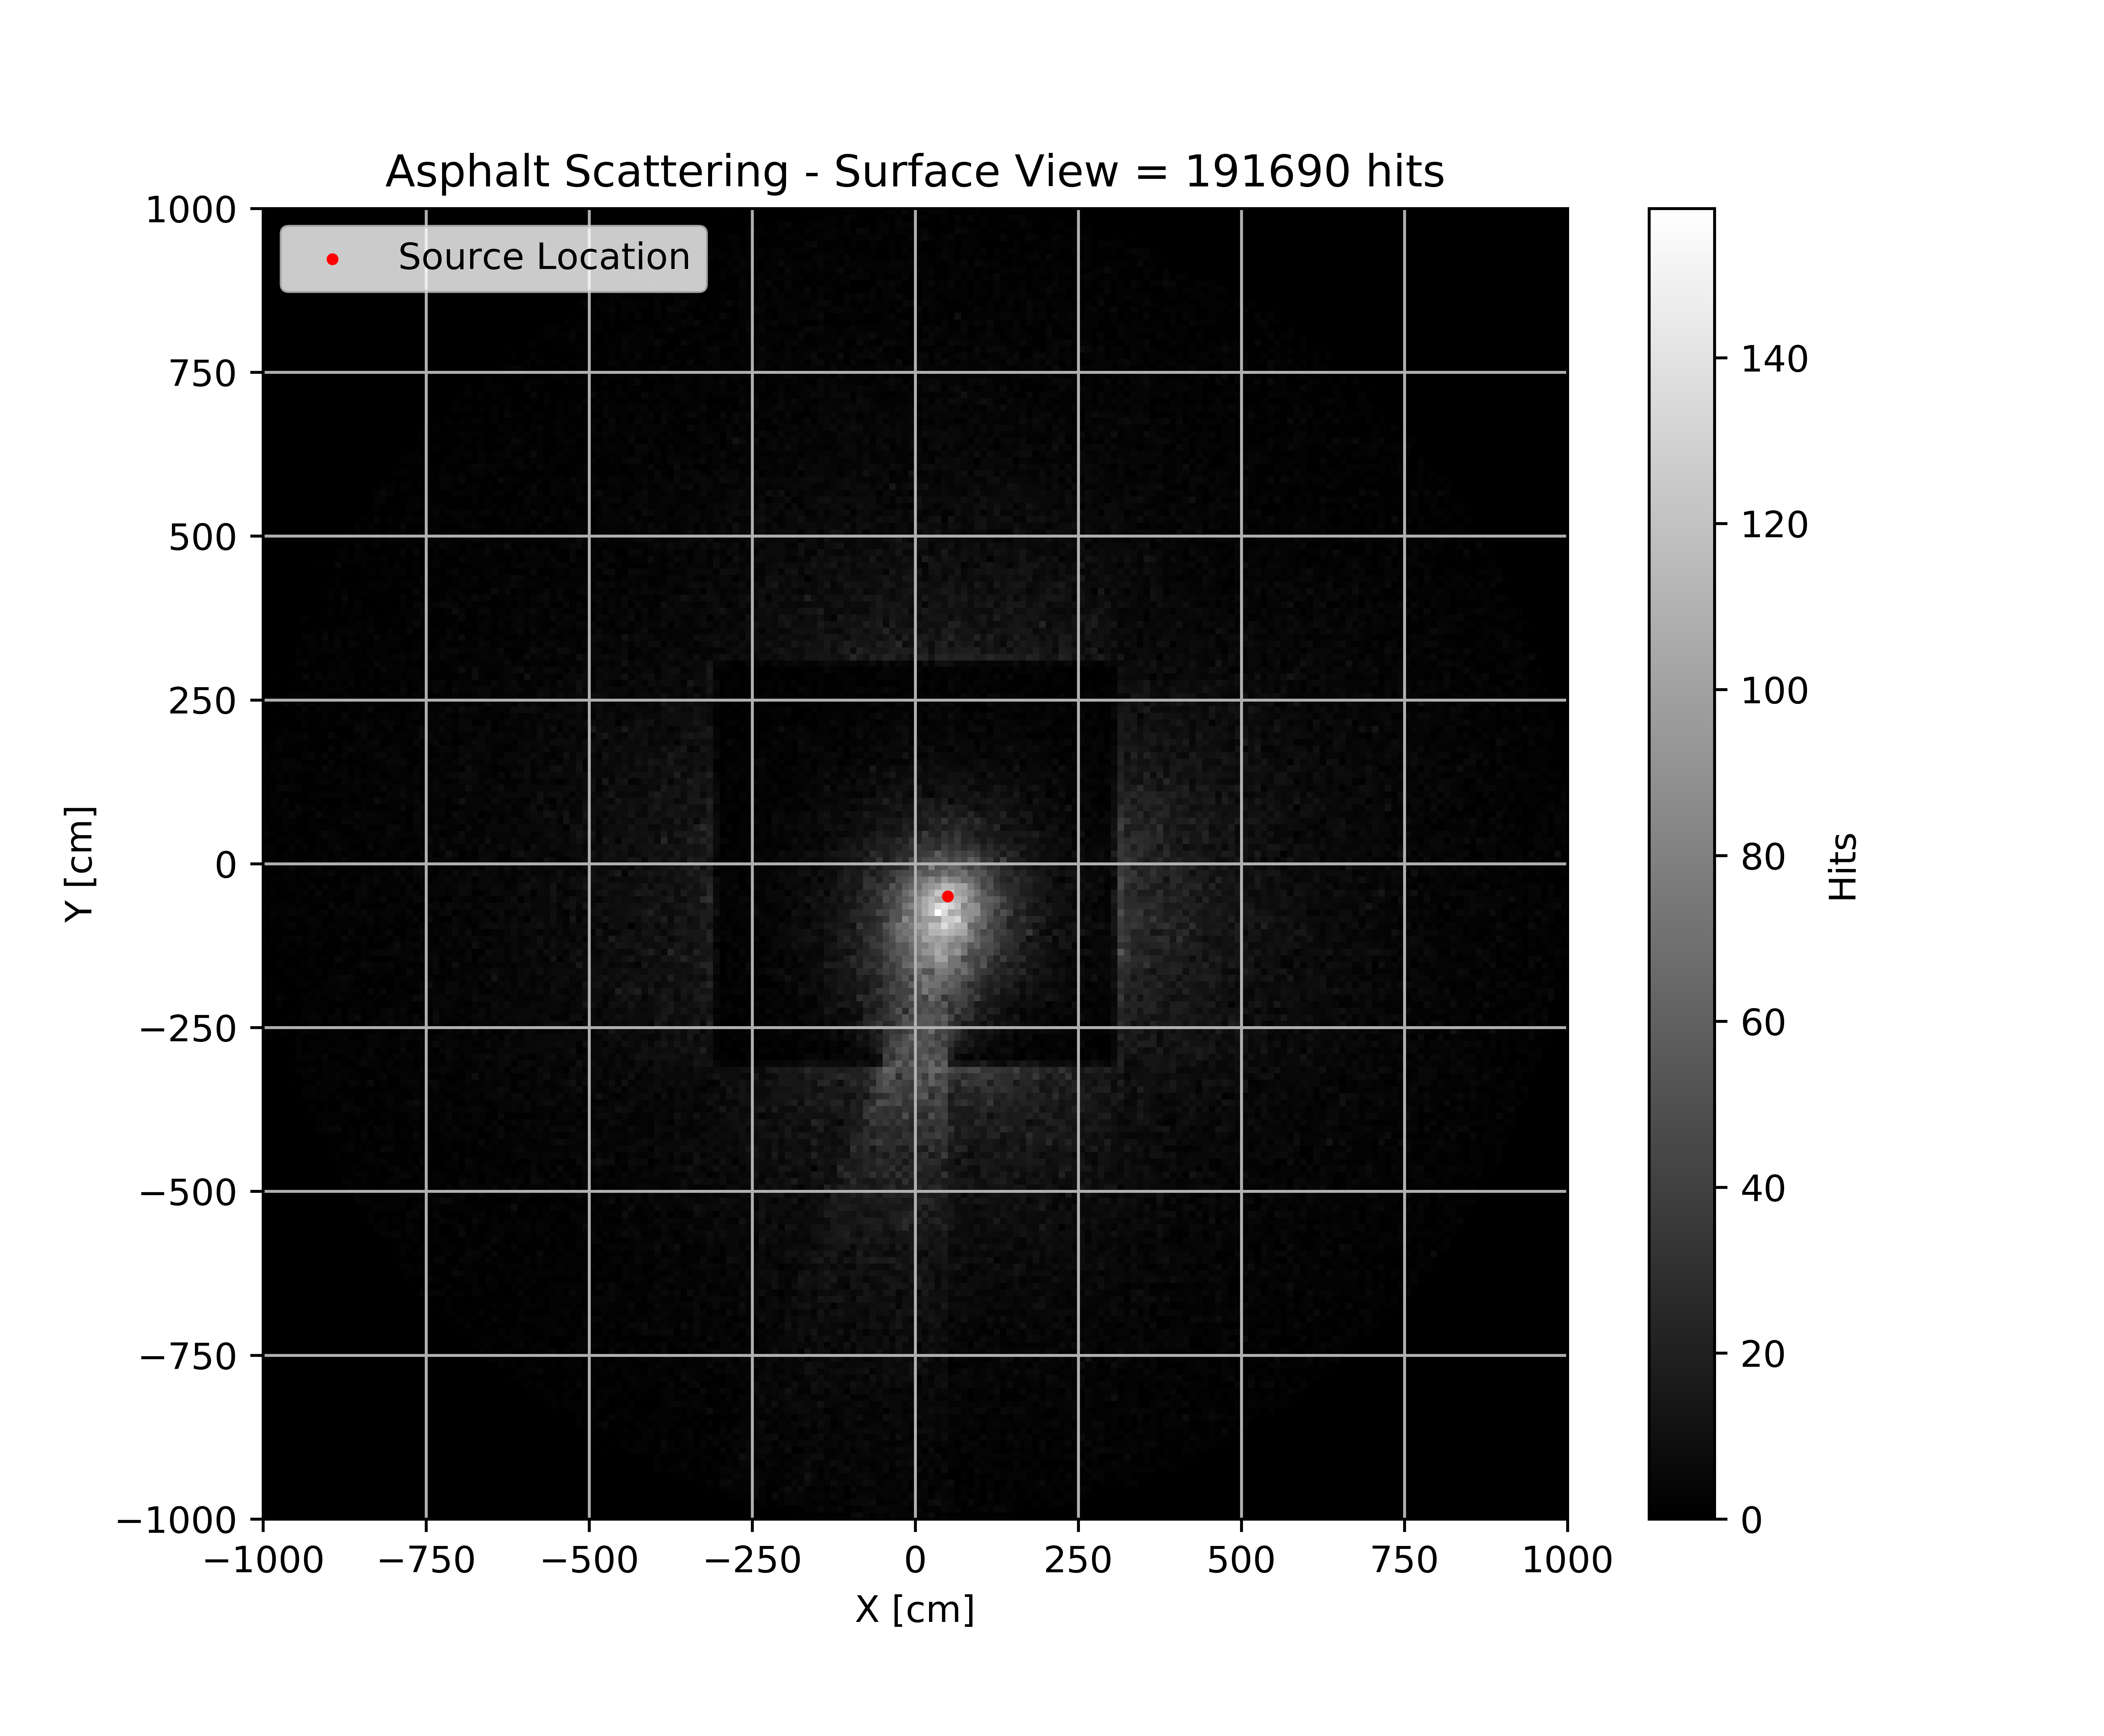
\includegraphics[width=\columnwidth]{images/10Asphalt_Scattered_1fl_cen}
  \caption{Ground flux due to gamma scattering off asphalt}
  \label{fig:AsScat1C}
\end{figure}

Fig. \ref{fig:AsScat1C} shows the ground flux due to gamma scattering off the asphalt. The unimpeded line of sight to the detector plane is clearly visible in this image.

\begin{figure}[!htb]
\begin{subfigure}[b]{0.55\textwidth}
   \centering
   \includegraphics[width=1\linewidth]{images/13Flux_South_Comparison_1fl_cen}
   \caption{}
   \label{fig:S1C}
\end{subfigure}
\begin{subfigure}[b]{0.55\textwidth}
   \centering
   \includegraphics[width=1\linewidth]{images/12Flux_North_Comparison_1fl_cen}
   \caption{}
   \label{fig:N1C}
\end{subfigure}
\caption{(a) The quantified flux as viewed from the South. (b) The quantified flux as viewed from the North.}
\end{figure}

\noindent This simulation clearly shows how an open door can assist in detection. Moreover, one would not expect to have more full energy hits than partial energy due to scattering when dealing with 10 cm concrete wall, however the open geometry gave the detector a large aperture with a direct line on sight.

\begin{figure}[!htb]
\begin{subfigure}[b]{0.55\textwidth}
   \centering
   \includegraphics[width=1\linewidth]{images/17_3D_Flux_Tot_1fl_cen}
   \caption{}
   \label{fig:3DT1C}
\end{subfigure}
\begin{subfigure}[b]{0.55\textwidth}
   \centering
   \includegraphics[width=1\linewidth]{images/17_3D_Flux_Full_1fl_cen}
   \caption{}
   \label{fig:3DF1C}
\end{subfigure}
\begin{subfigure}[b]{0.55\textwidth}
   \centering
   \includegraphics[width=1\linewidth]{images/17_3D_Flux_Part_1fl_cen}
   \caption{}
   \label{fig:3DP1C}
\end{subfigure}
\caption{(a) 3D quantified total flux as viewed from the Southeast. (b) 3D quantified full energy flux as viewed from the Southeast. (c) 3D quantified partial energy flux as viewed from the Southeast.}
\end{figure}

Figs. \ref{fig:3DT1C}, \ref{fig:3DF1C}, and \ref{fig:3DP1C} show 3D depictions of the quantified flux. Fig. \ref{fig:3DF1C} has no ground plane because all gammas traced back to the asphalt were scattering events that resulted in a loss of energy.

\subsection{Localization}
\noindent The following results are from the source located on the second floor in position closest to the wall as described in Table \ref{table:positions}.

\begin{figure}[!htb]
\begin{subfigure}[b]{0.5\textwidth}
   \centering
   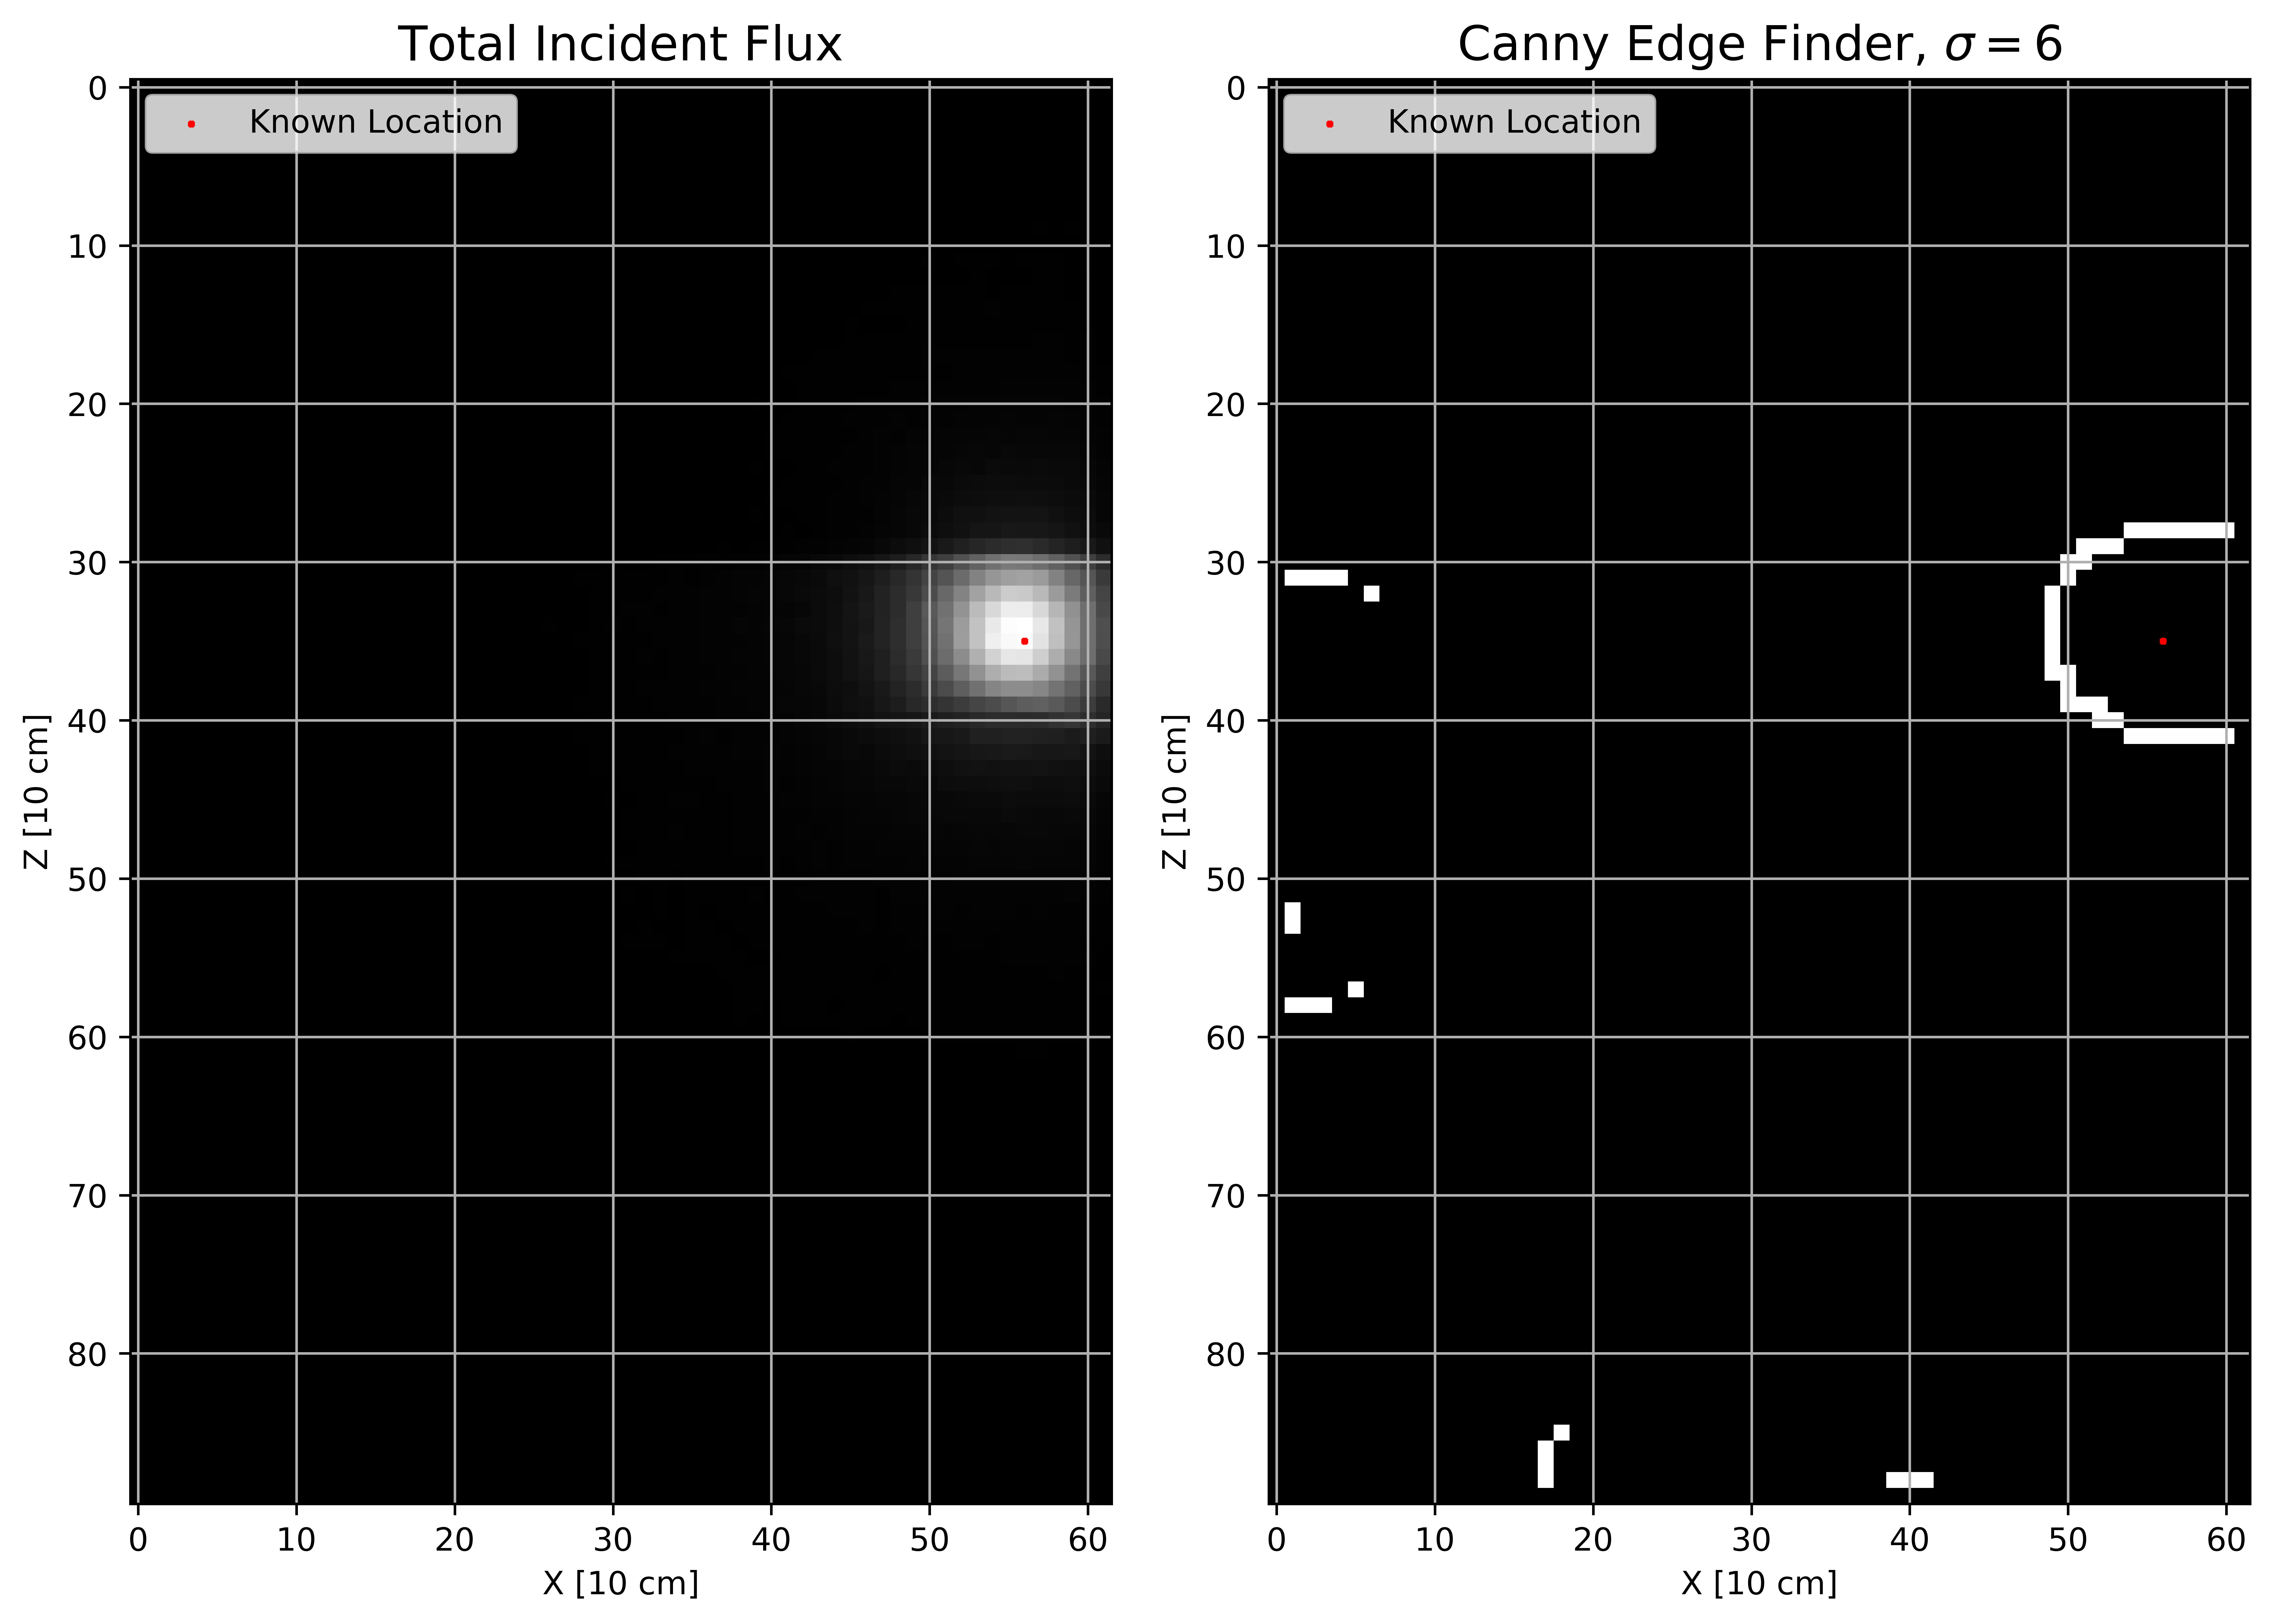
\includegraphics[width=1\linewidth]{images/1Canny_Total_2fl_Wall_S}
   \caption{}
   \label{fig:Can2FTotS}
\end{subfigure}
\begin{subfigure}[b]{0.5\textwidth}
   \centering
   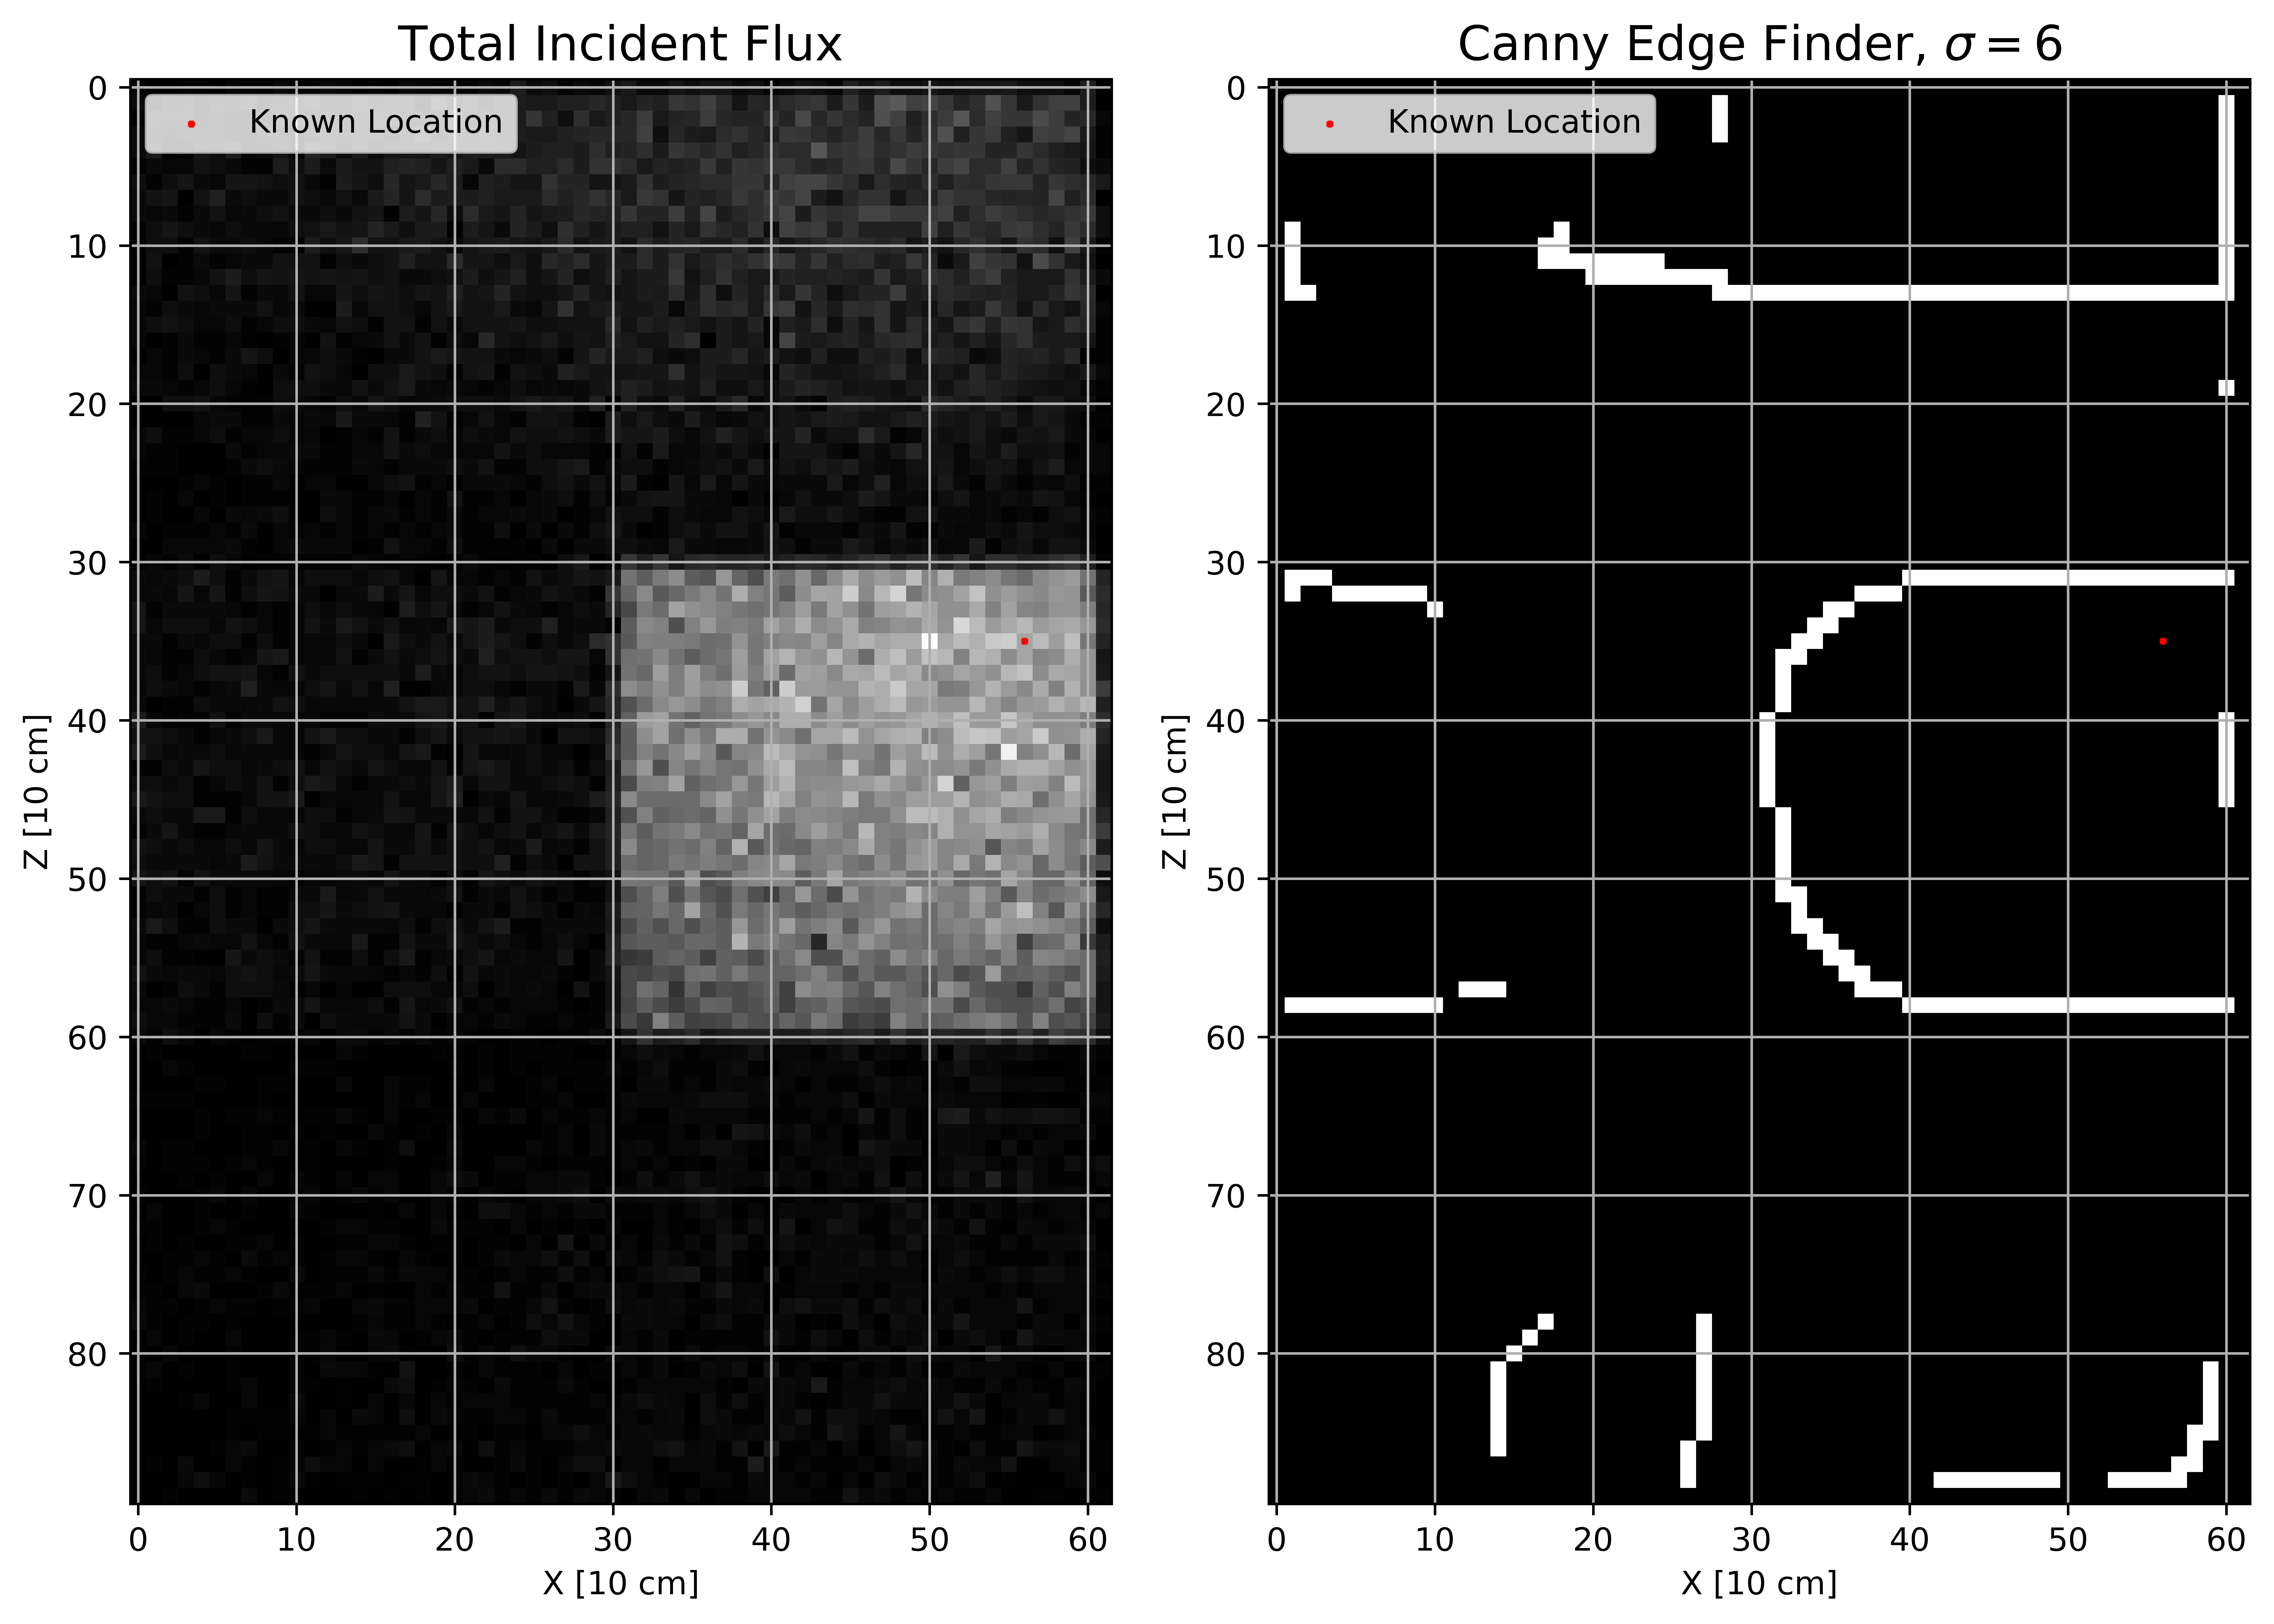
\includegraphics[width=1\linewidth]{images/1Canny_Total_2fl_Wall_N}
   \caption{}
   \label{fig:Can2FTotN}
\end{subfigure}
\caption{(a) The quantified total flux and 6$\sigma$ Canny filter as viewed from the South. (b) The quantified total flux and 6$\sigma$ Canny filter as viewed from the North.}
\end{figure}

\noindent Figs. \ref{fig:Can2FTotS} and \ref{fig:Can2FTotN} show the first step of localization, implementing a Canny edge finder. Fig. \ref{fig:Can2FTotS} also demonstrates how the closer a source is to a surface, the more concentrated the flux distribution, which can lead to more precise localization. Fig. \ref{fig:Can2FTotN} demonstrates how a building's construction, in this case internal walls, can assist in localization by limiting excess gamma transmission.

\begin{figure}[!htb]
\begin{subfigure}[b]{0.15\textwidth}
   \centering
   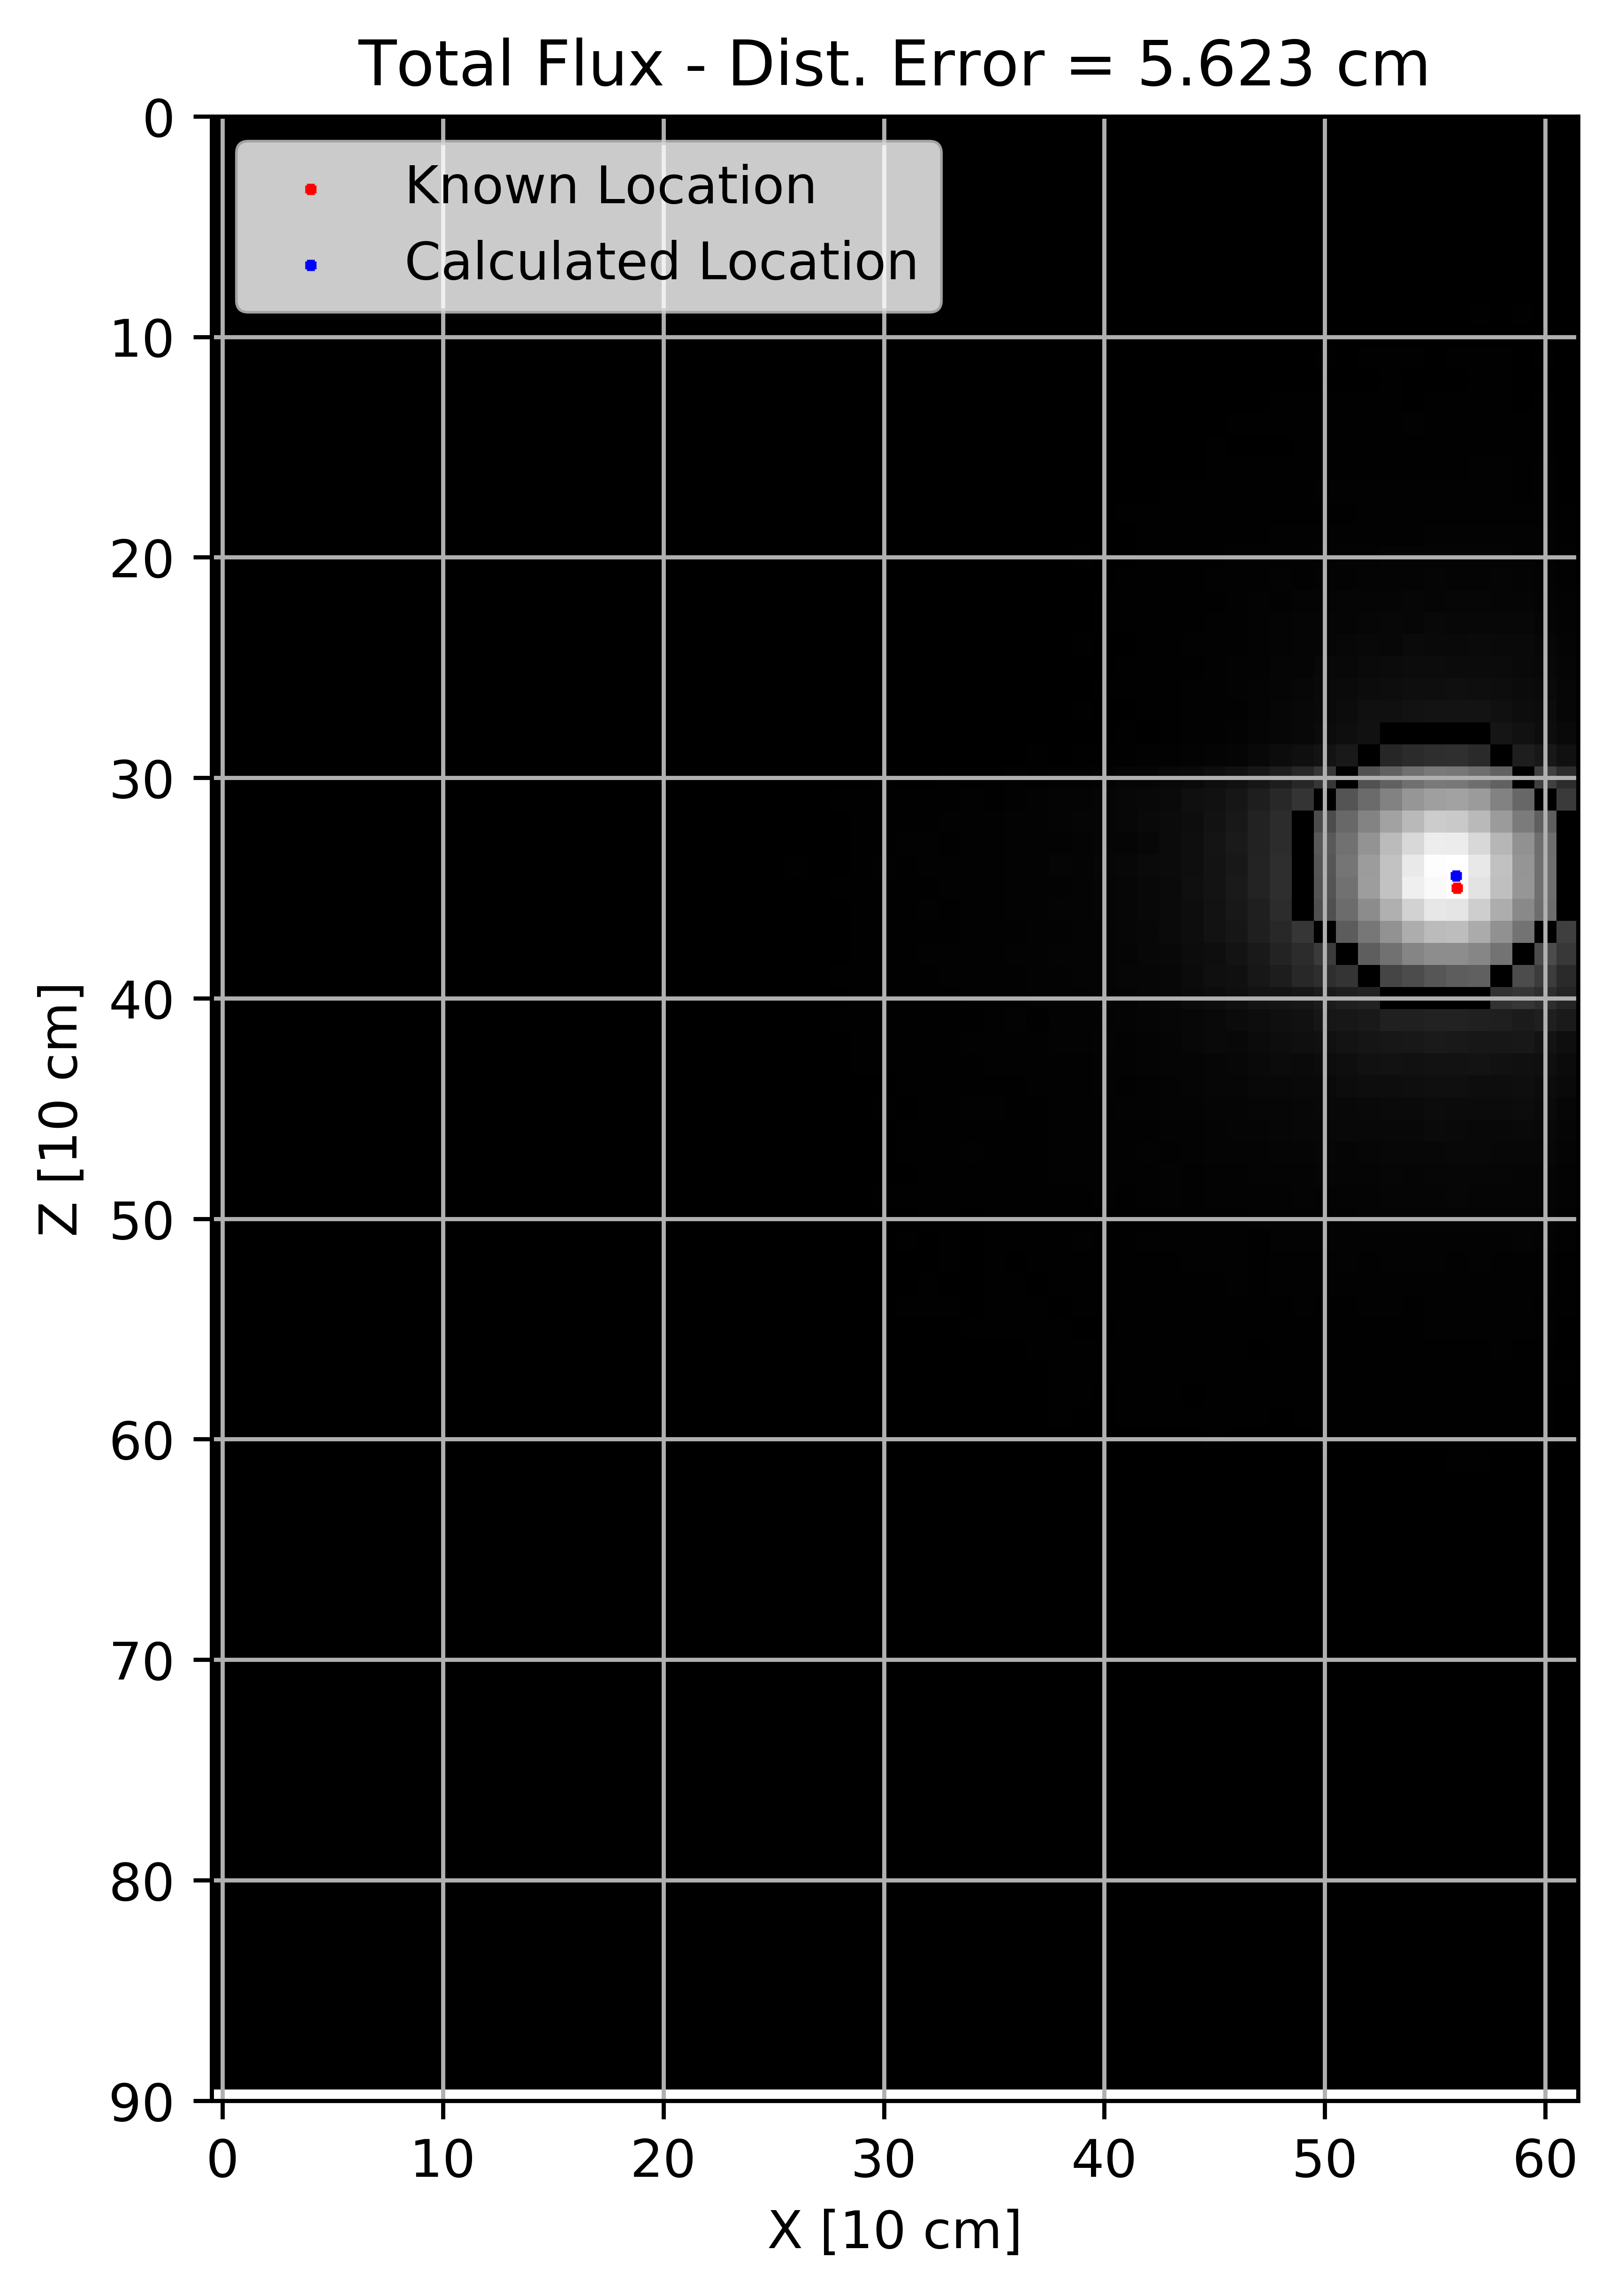
\includegraphics[width=1\linewidth]{images/2Cent_Total_2fl_Wall_S}
   \caption{}
   \label{fig:RanT2W}
\end{subfigure}
\begin{subfigure}[b]{0.15\textwidth}
   \centering
   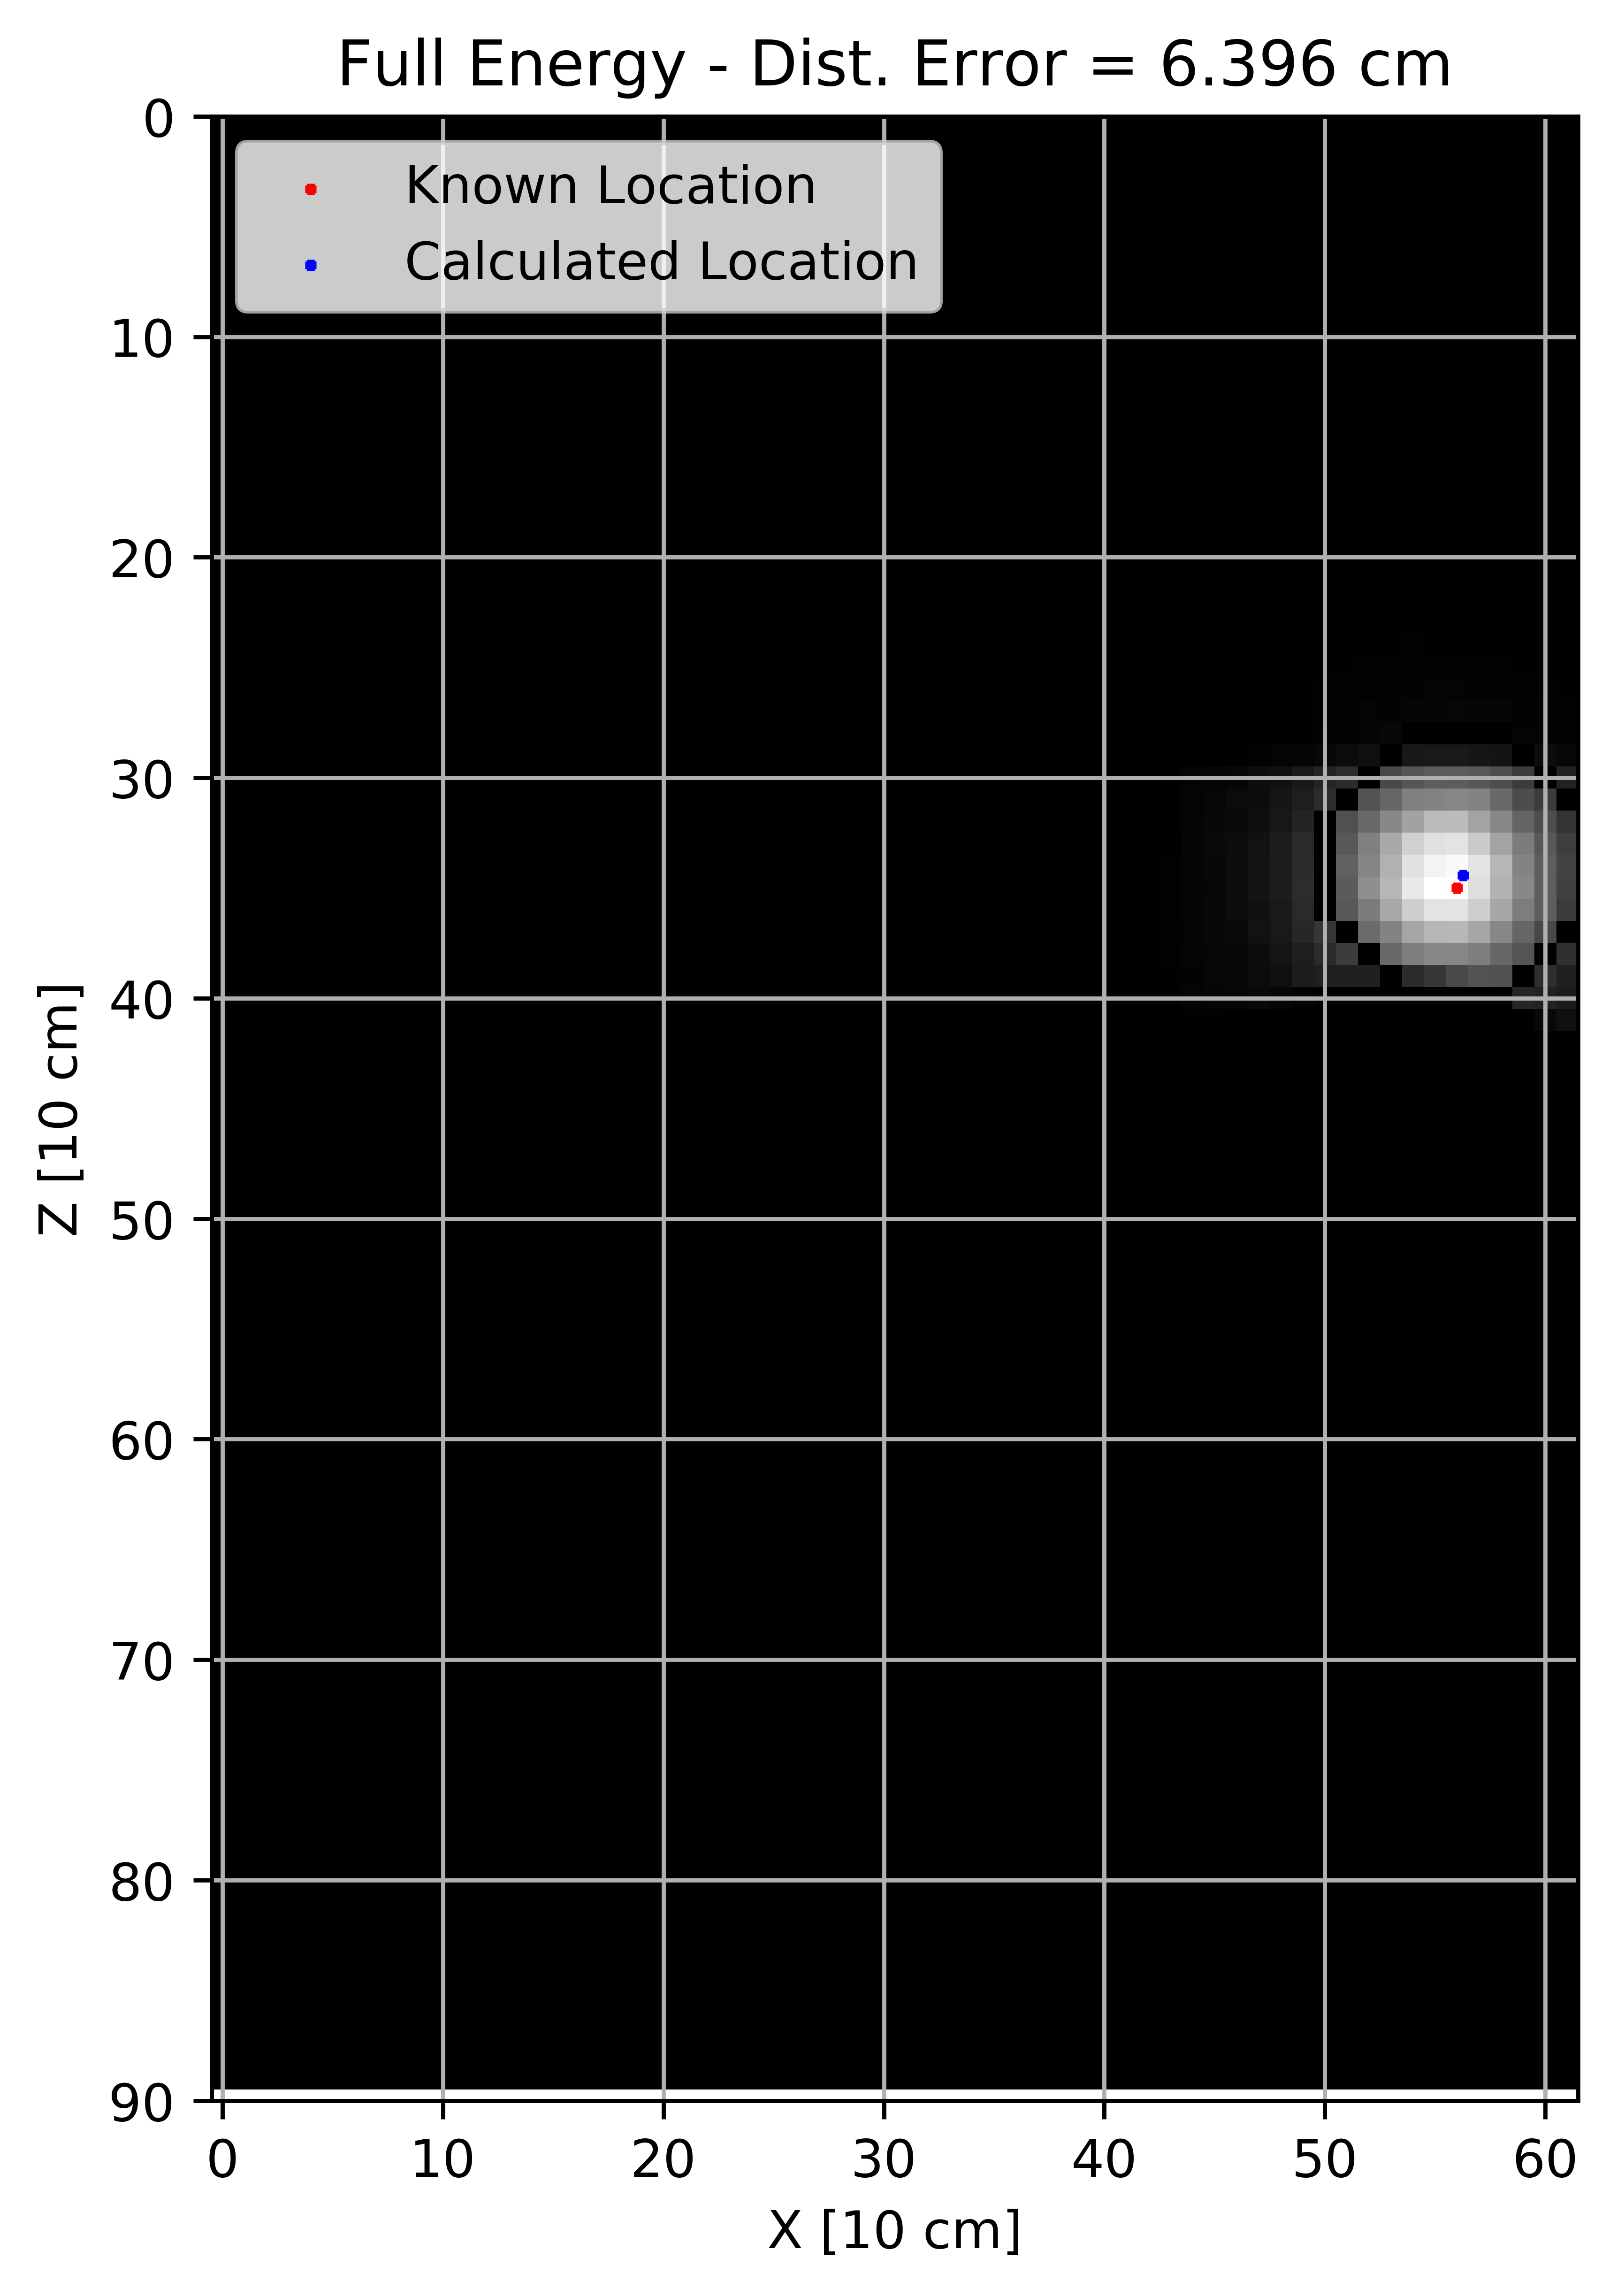
\includegraphics[width=1\linewidth]{images/2Cent_Full_2fl_Wall_S}
   \caption{}
   \label{fig:RanF2W}
\end{subfigure}
\begin{subfigure}[b]{0.15\textwidth}
   \centering
   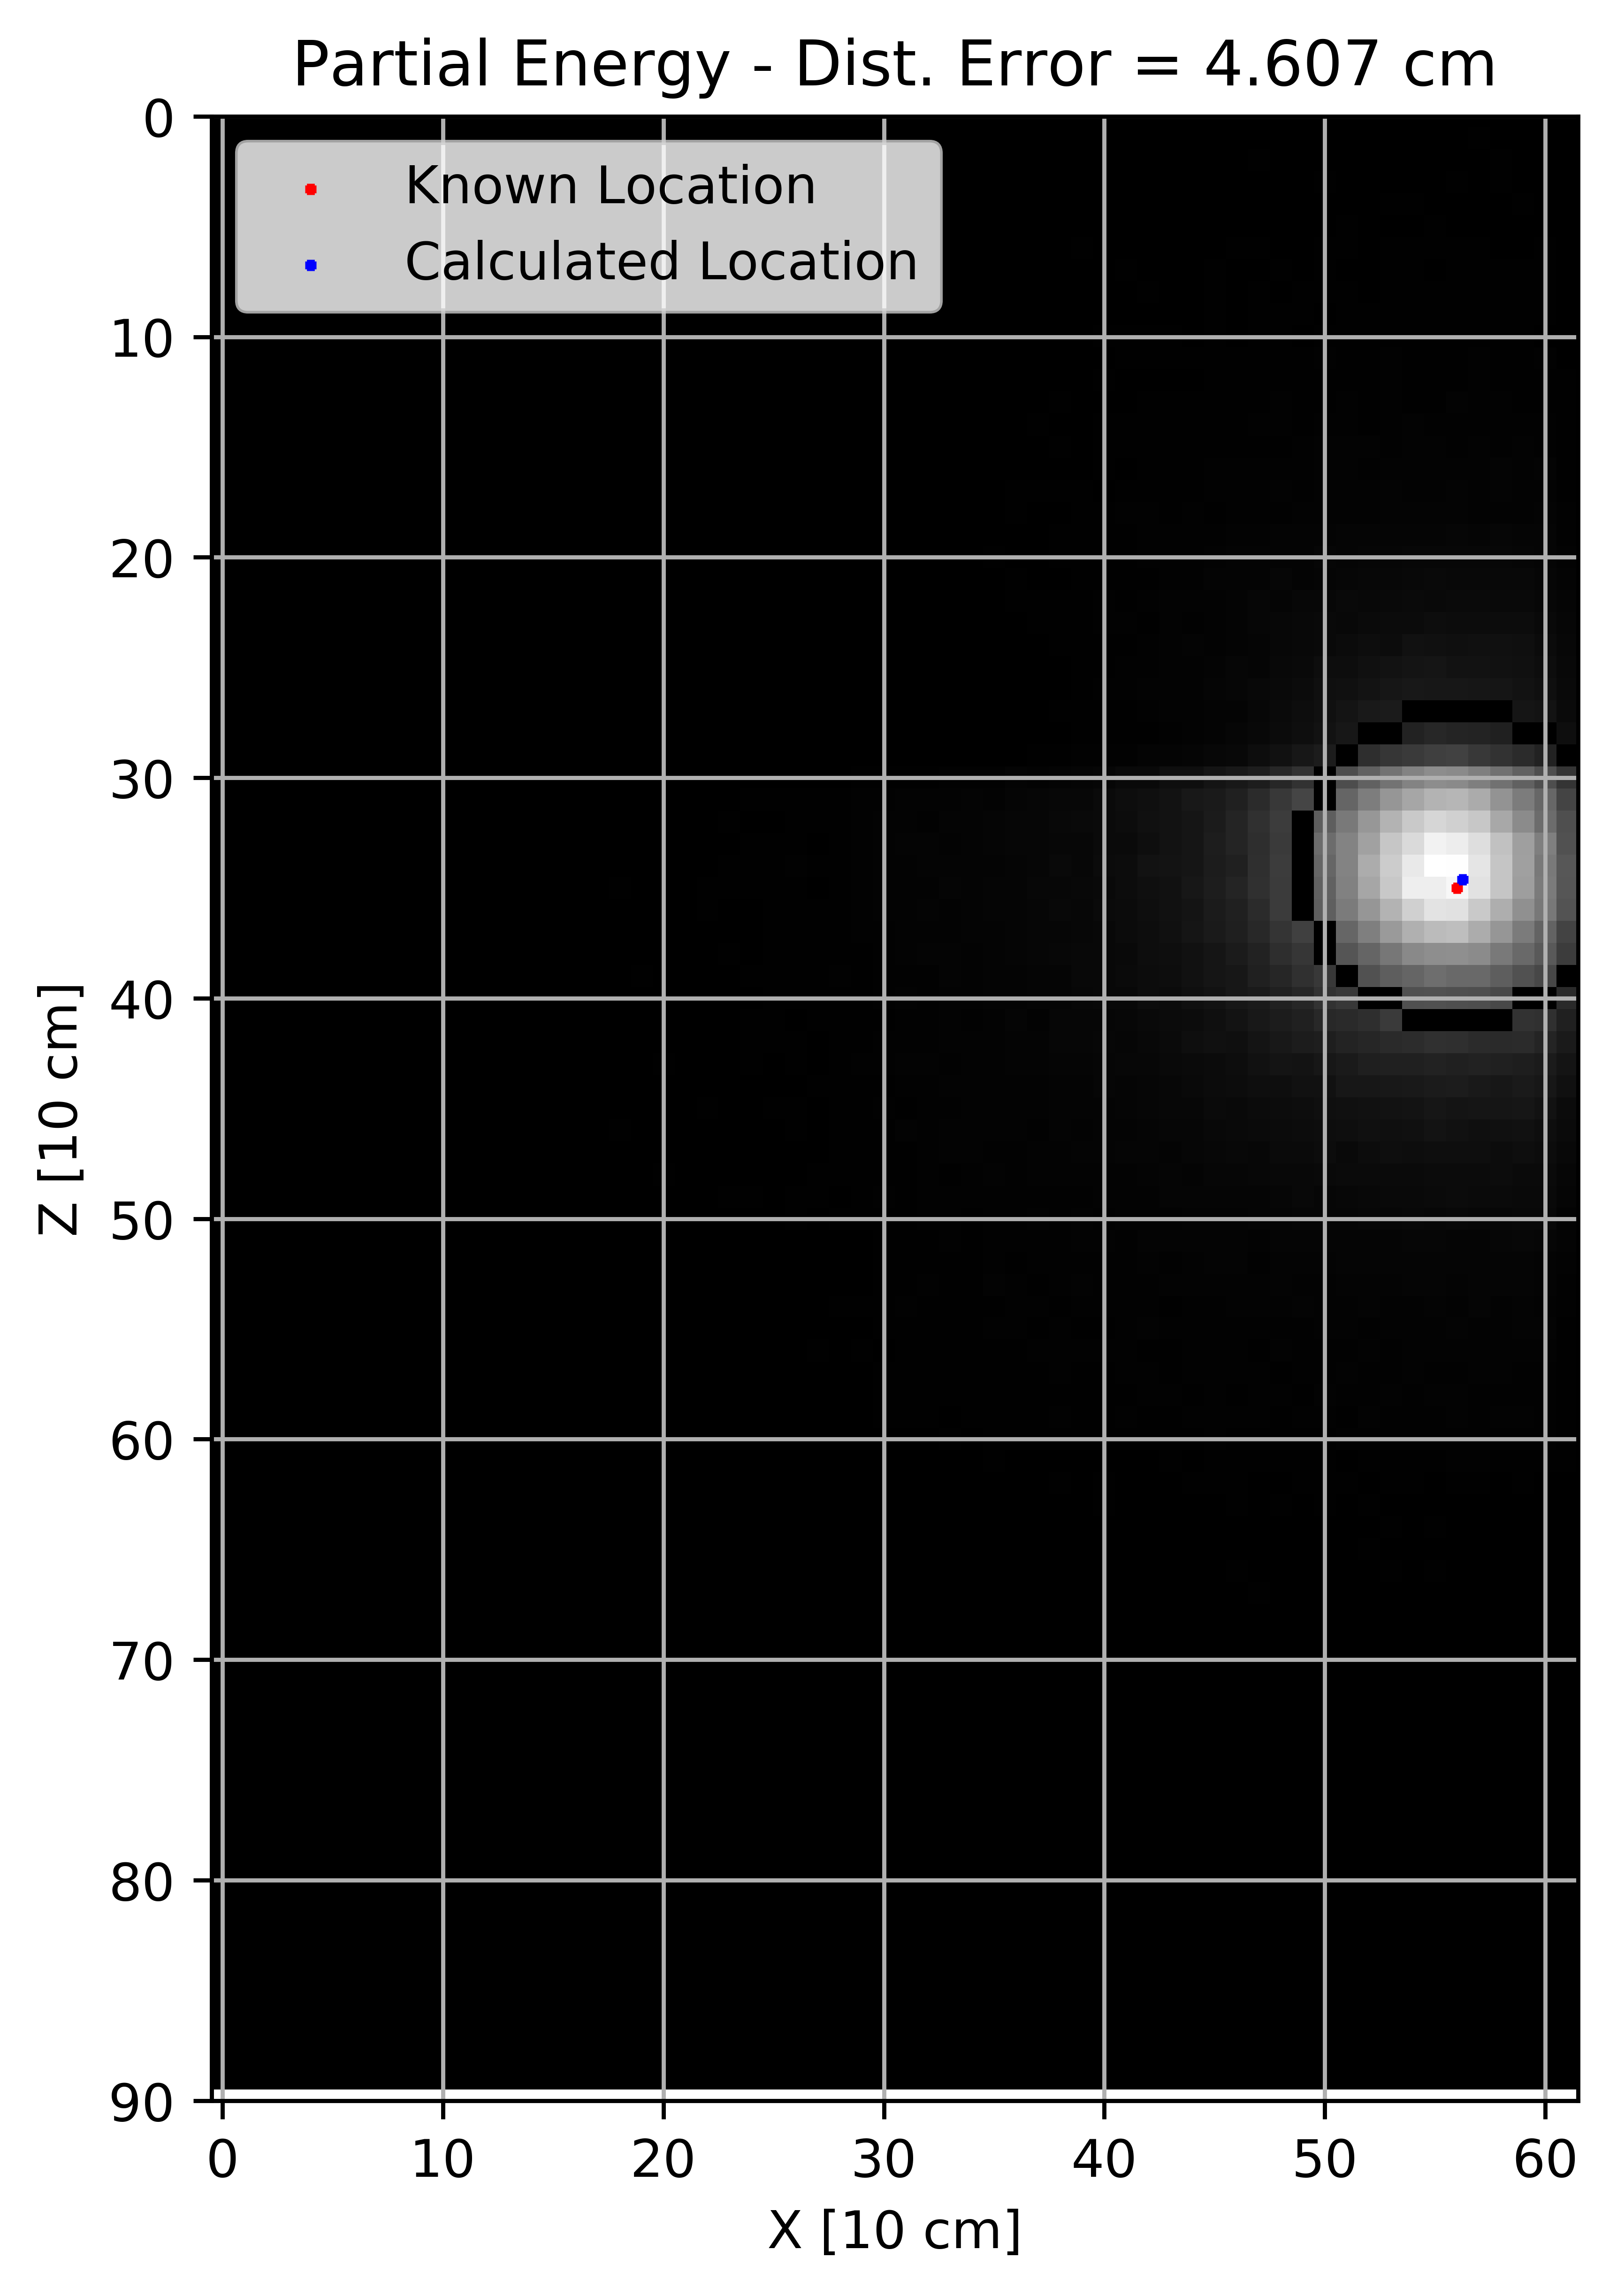
\includegraphics[width=1\linewidth]{images/2Cent_Part_2fl_Wall_S}
   \caption{}
   \label{fig:RanP2W}
\end{subfigure}
\caption{(a) Estimated source location using total flux from South. (b) Estimated source location using full energy flux from South. (c) Estimated source location using partial flux from South.}
\end{figure}

\begin{figure}[!htb]
\begin{subfigure}[b]{0.15\textwidth}
   \centering
   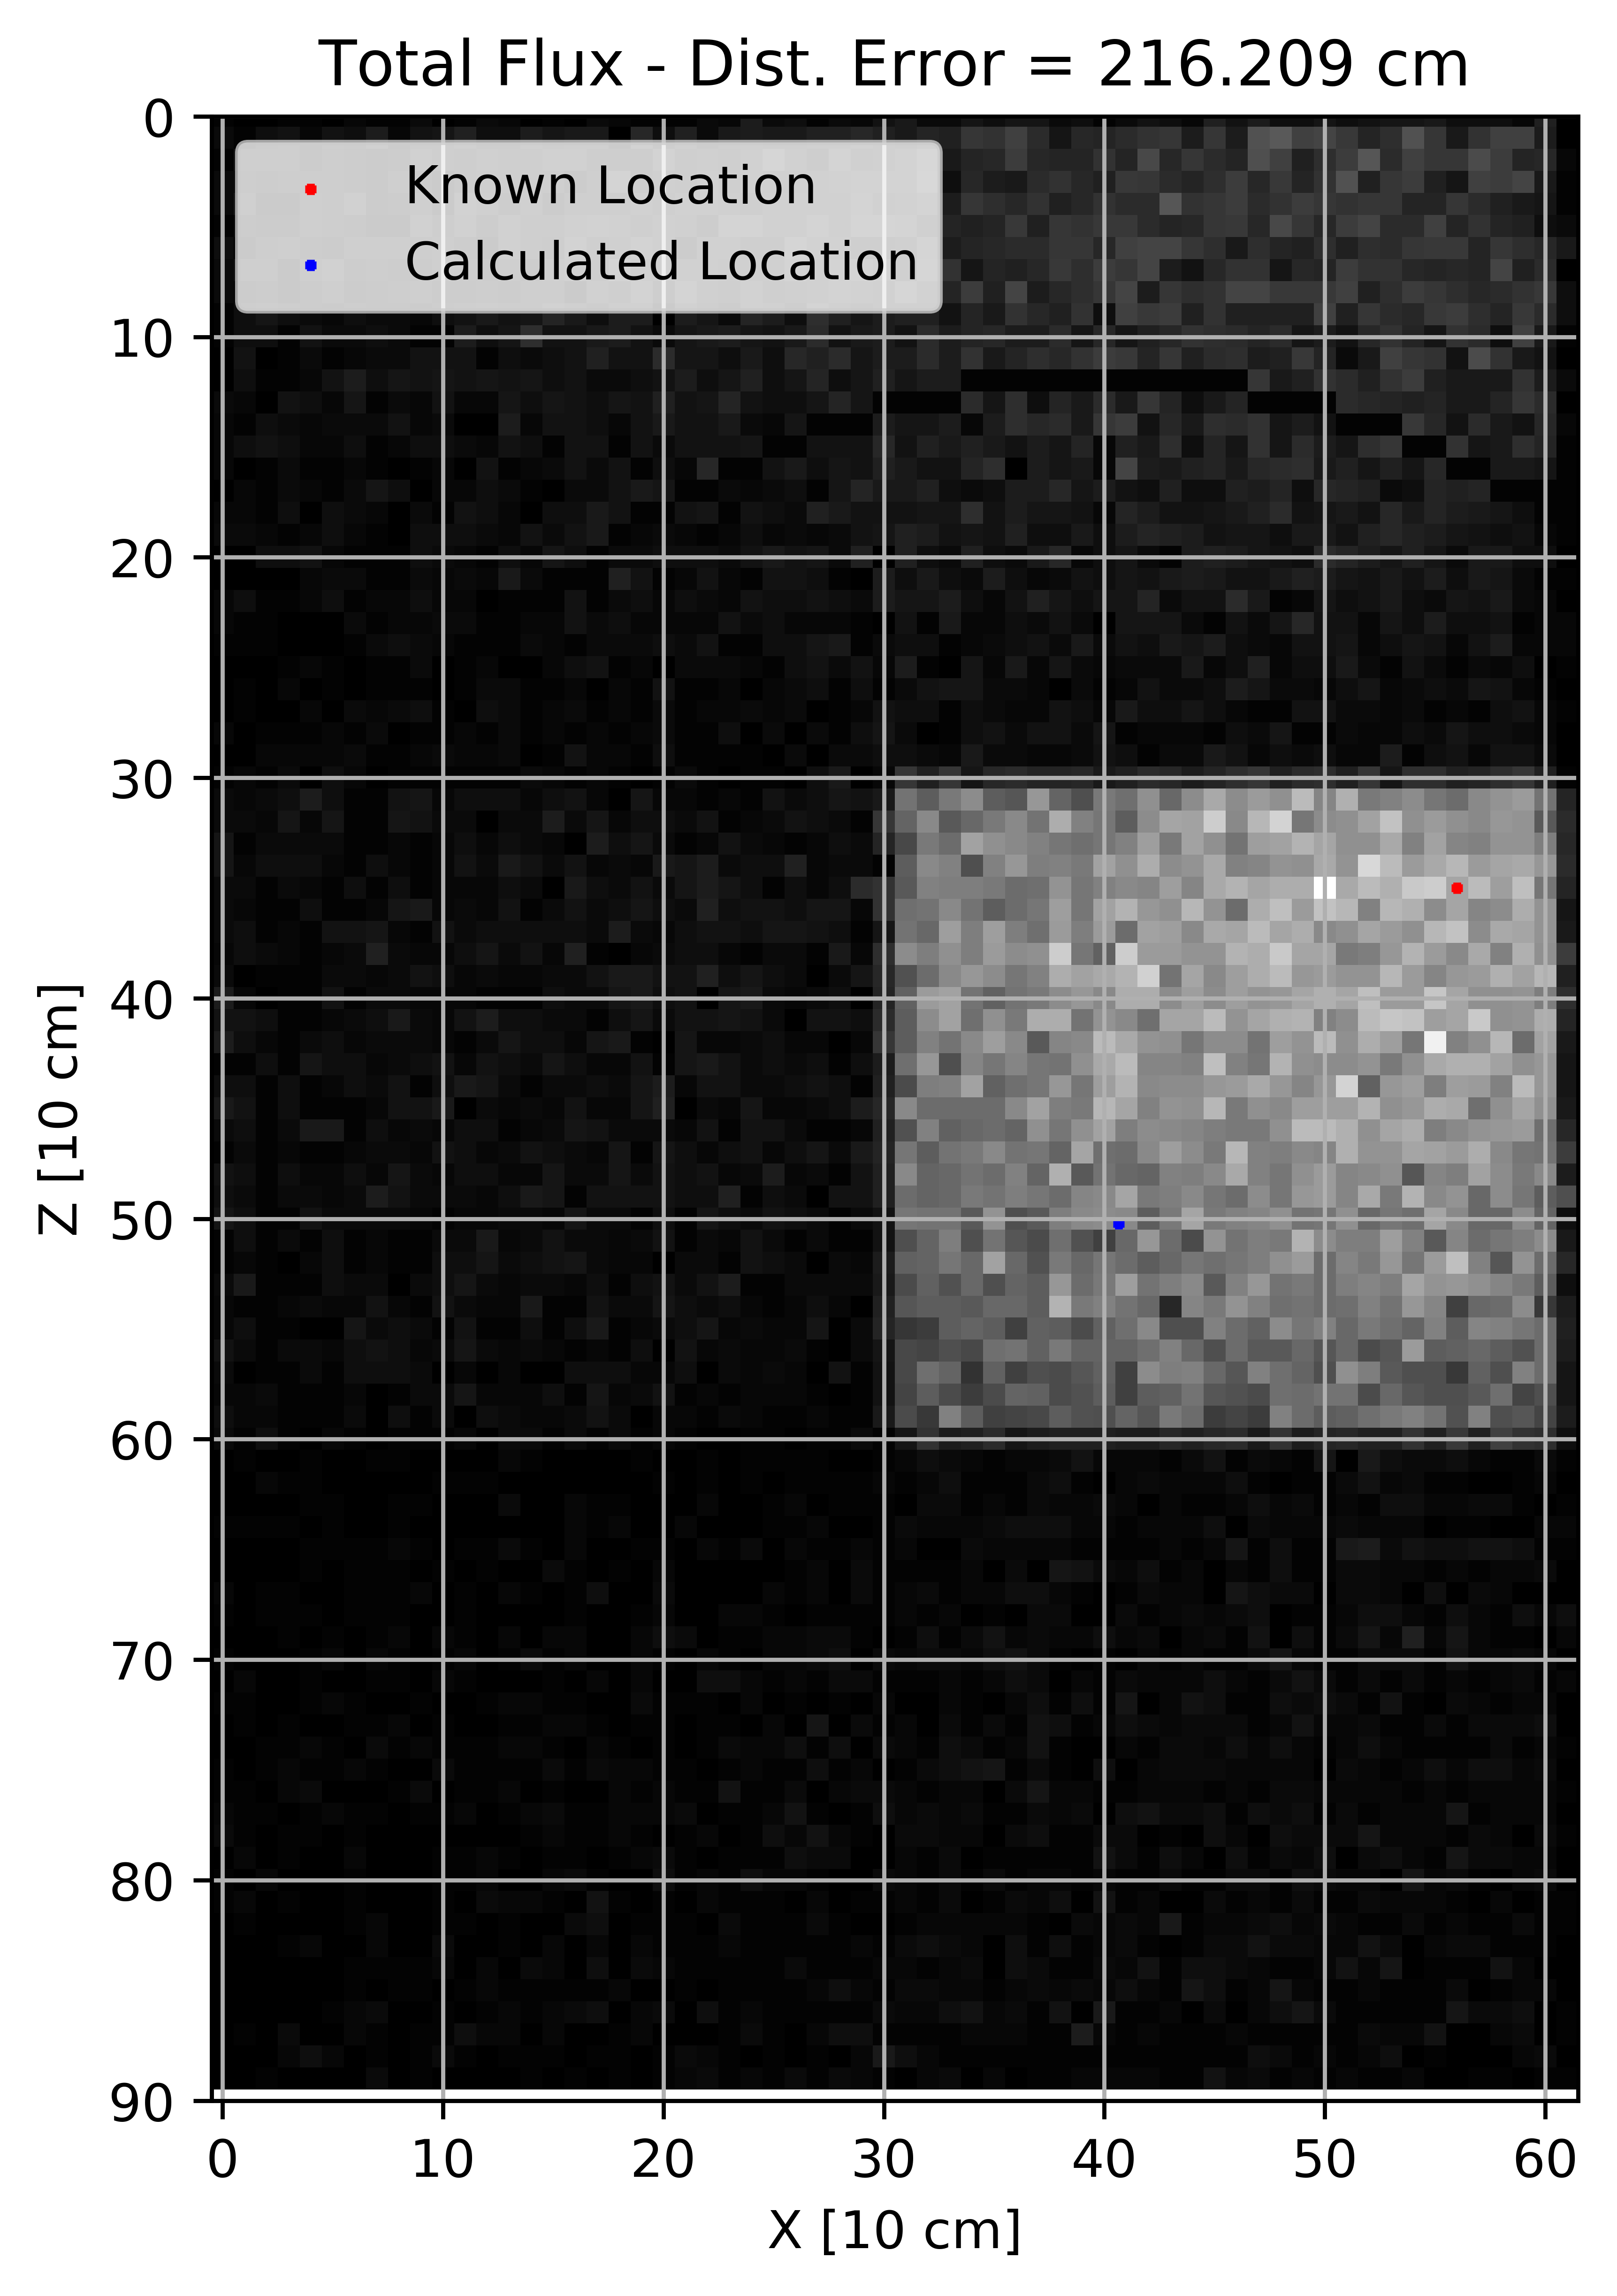
\includegraphics[width=1\linewidth]{images/2Cent_Total_2fl_Wall_N}
   \caption{}
   \label{fig:RanT2WN}
\end{subfigure}
\begin{subfigure}[b]{0.15\textwidth}
   \centering
   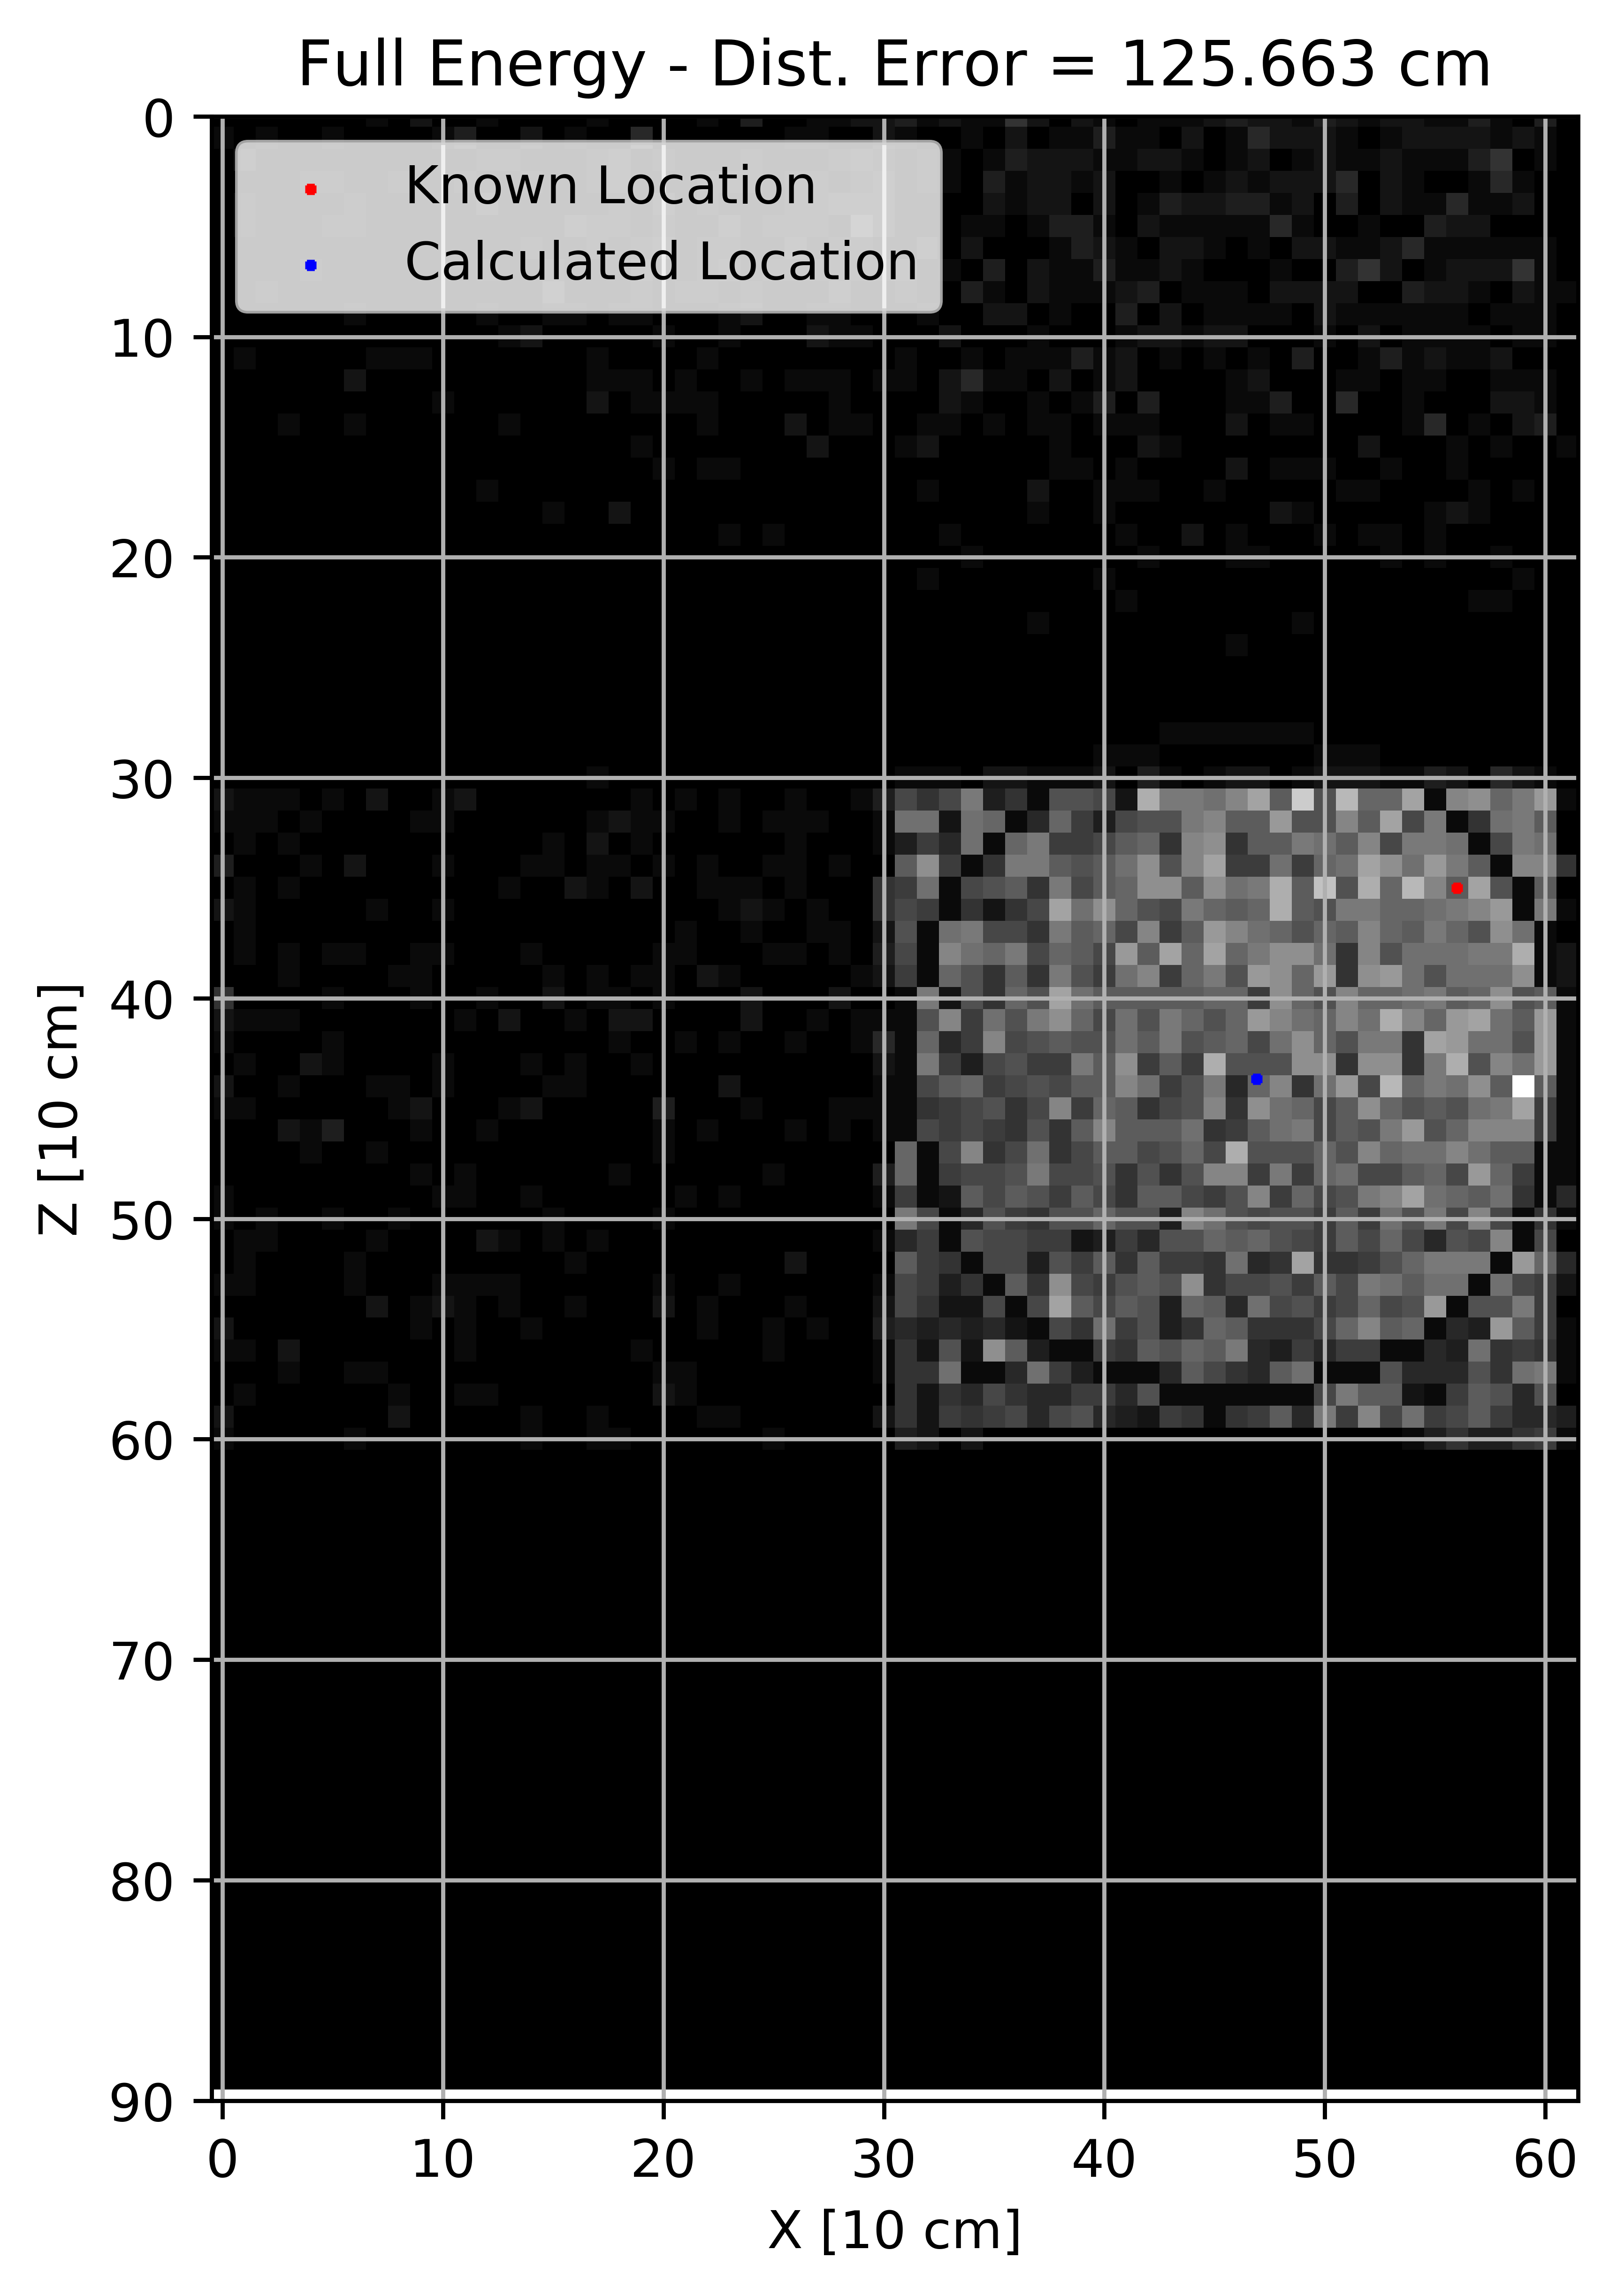
\includegraphics[width=1\linewidth]{images/2Cent_Full_2fl_Wall_N}
   \caption{}
   \label{fig:RanF2WN}
\end{subfigure}
\begin{subfigure}[b]{0.15\textwidth}
   \centering
   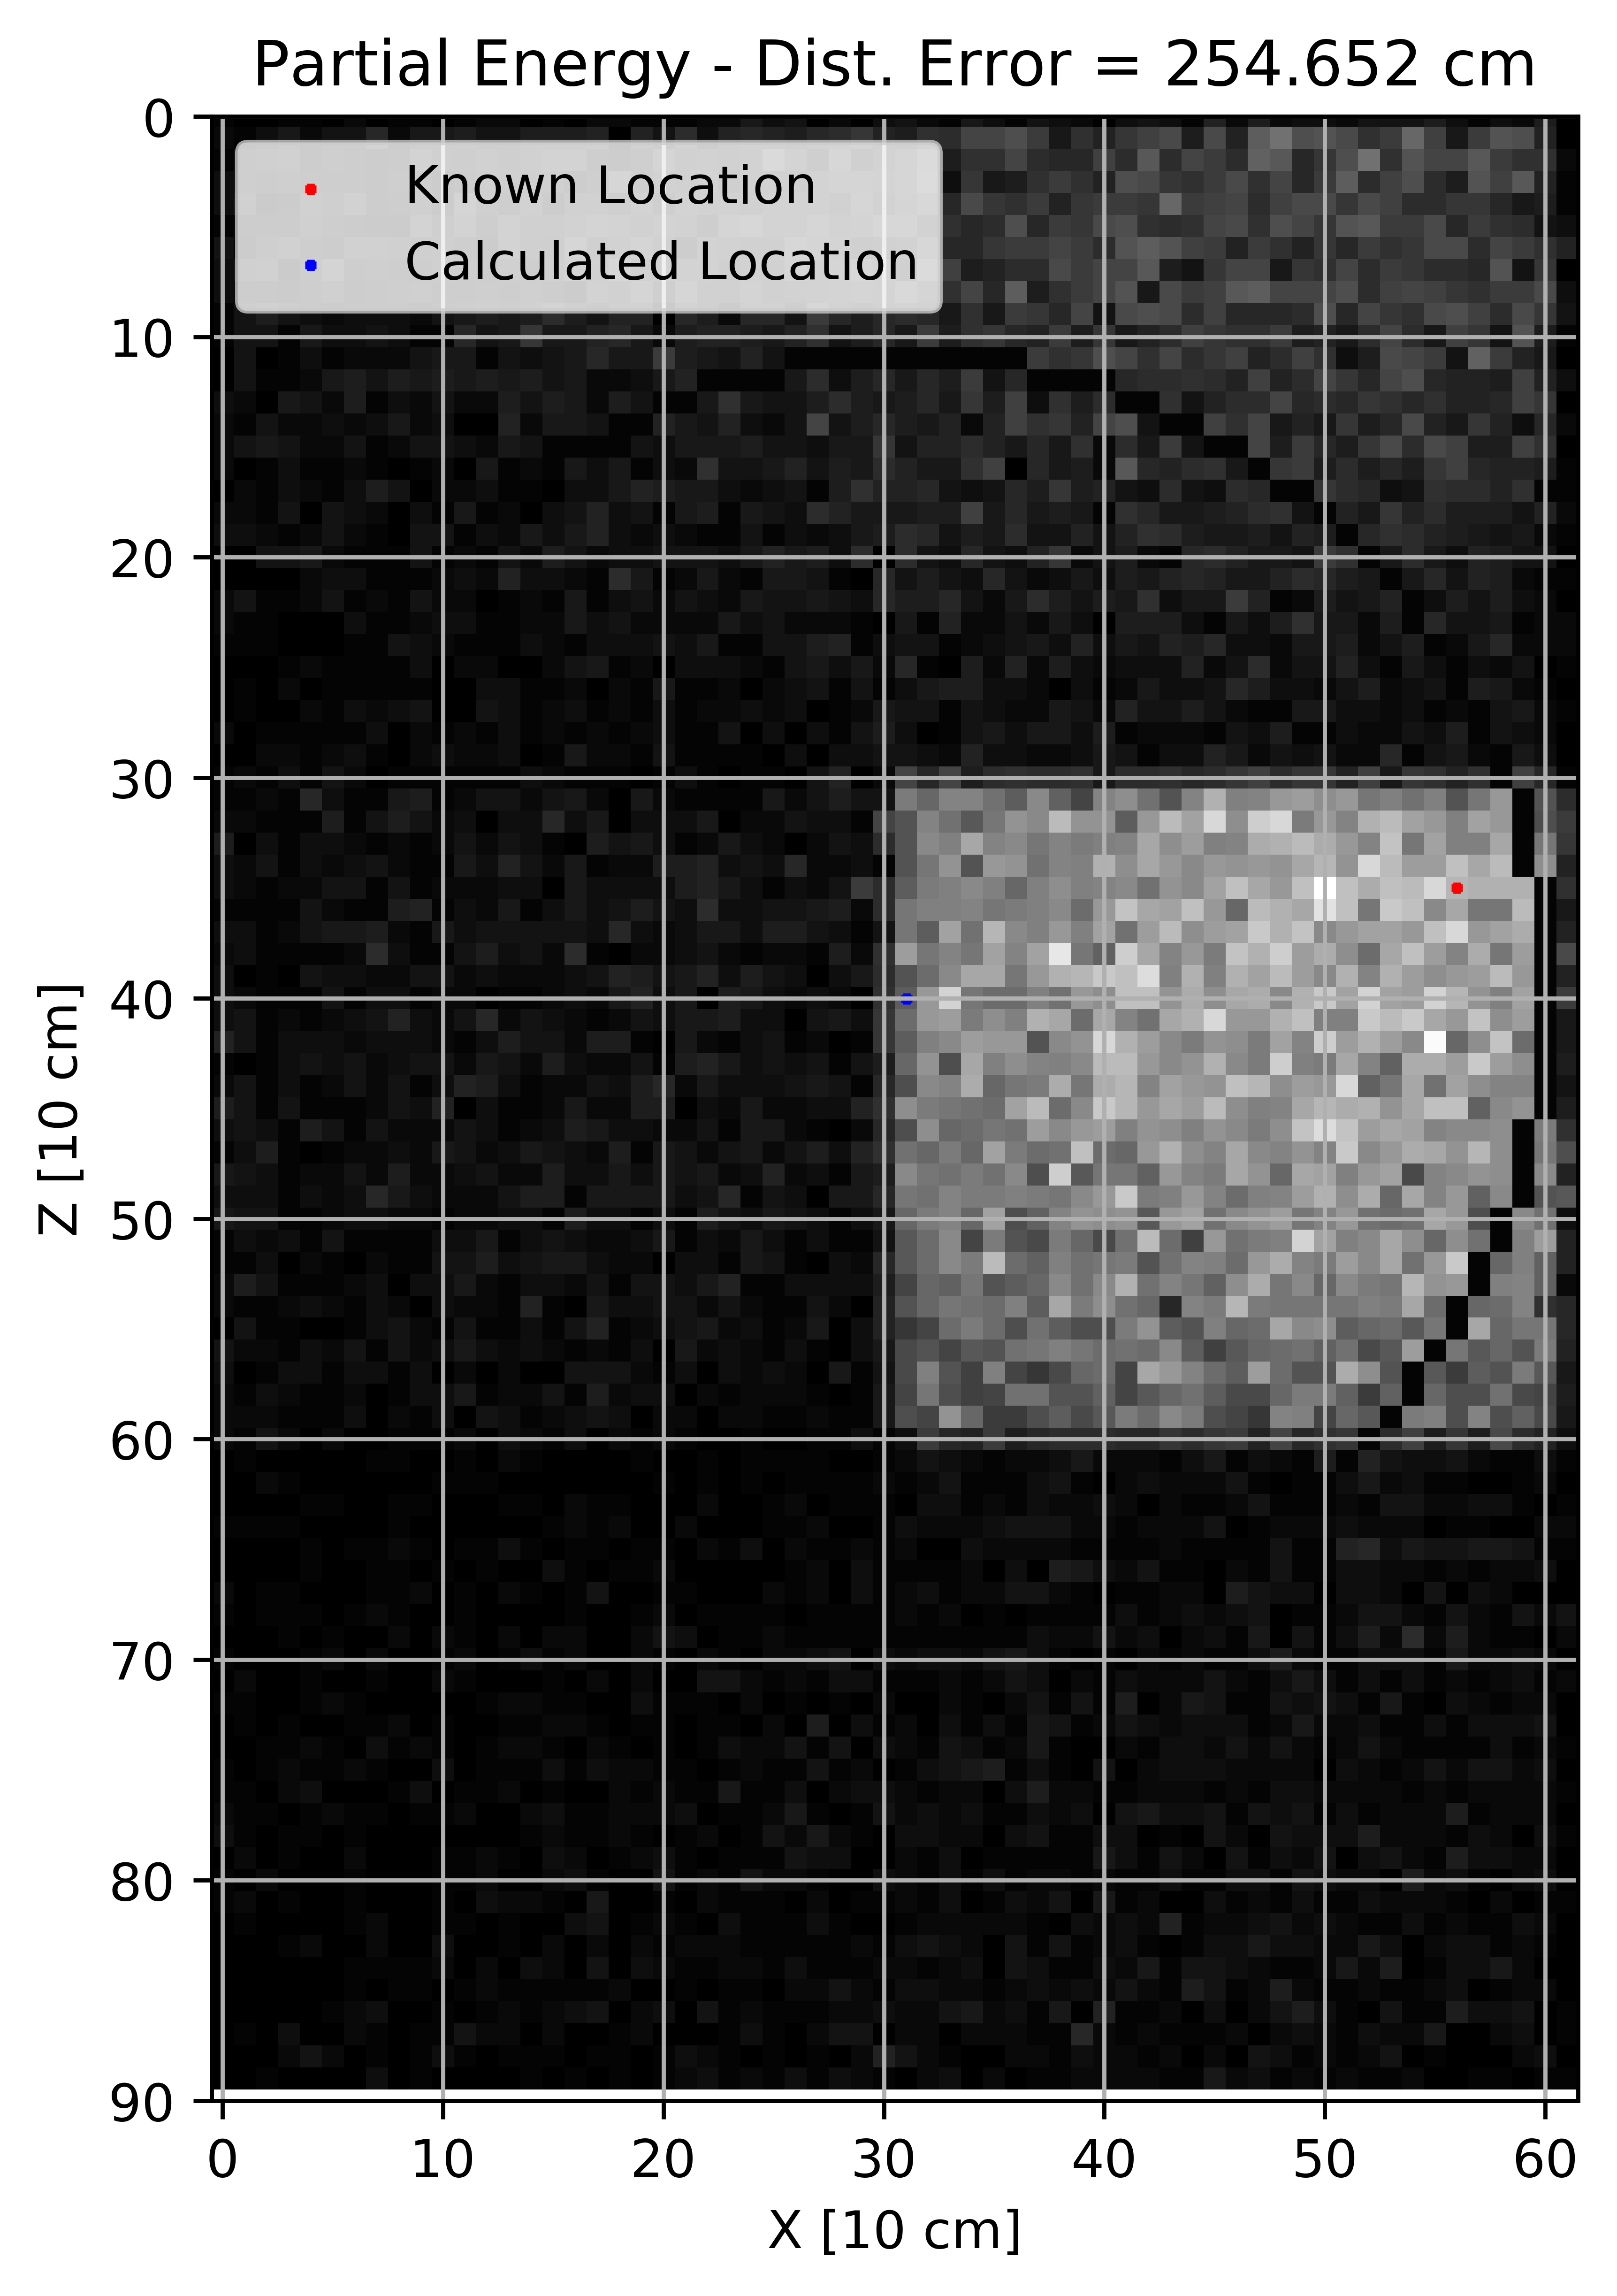
\includegraphics[width=1\linewidth]{images/2Cent_Part_2fl_Wall_N}
   \caption{}
   \label{fig:RanP2WN}
\end{subfigure}
\caption{(a) Estimated source location using total flux from North. (b) Estimated source location using full energy flux from North. (c) Estimated source location using partial flux from North.}
\end{figure}

\noindent Figs. \ref{fig:RanT2W}, \ref{fig:RanF2W}, and \ref{fig:RanP2W} all show an accuracy of less than 7 cm, this is particularly impressive given the detector distance from the source and 10 cm of concrete. However, Figs. \ref{fig:RanT2WN}, \ref{fig:RanF2WN}, and \ref{fig:RanP2WN} show how it can be hard to localize from the far side of the building and how the radial dispersion of total and partial flux lead to larger lateral error.
\\\\
\begin{table}[!htp]
 \caption{Error in Estimated Source Location}
  \begin{center}
    \begin{tabulary}{\columnwidth}{cccc}
      \hline
      Floor & Location & Response & Error [cm] \\ \hline
      1 & Central & Total & 165.76 \\
      1 & Central & Full E & 92.95\\
      1 & Central & Partial E & 173.09 \\
      1 & Middle & Total & 138.86 \\
      1 & Middle & Full E & 54.52 \\
      1 & Middle & Partial E & 100.95 \\
      1 & Wall & Total & 394.93 \\
      1 & Wall & Full E & 30.22 \\
      1 & Wall & Partial E & 354.67 \\
      2 & Central & Total & 134.64 \\
      2 & Central & Full E & 101.34 \\
      2 & Central & Partial E & 149.89 \\
      2 & Middle & Total & 36.30 \\
      2 & Middle & Full E & 79.29 \\
      2 & Middle & Partial E & 48.54 \\
      2 & Wall & Total & 316.12 \\
      2 & Wall & Full E & 7.43\\
      2 & Wall & Partial E & 51.54 \\
      3 & Central & Total & 89.33 \\
      3 & Central & Full E & 37.25 \\
      3 & Central & Partial E & 99.52 \\
      3 & Middle & Total & 36.14 \\
      3 & Middle & Full E & 23.86 \\
      3 & Middle & Partial E & 36.91 \\
      3 & Wall & Total & 361.73 \\
      3 & Wall & Full E & 36.40 \\
      3 & Wall & Partial E & 385.27 \\\hline
    \end{tabulary}
  \end{center}
  \label{table:error}
\end{table}

Table \ref{table:error} shows the location error for all nine simulations. In all but one scenario the gating on the peak energy yields a marked improvement over gross counts and partial energy counts. The best case estimated the source within 8 cm of its actual location.

\begin{table}[!htp]
 \caption{Mean Error by Response}
  \begin{center}
    \begin{tabulary}{\columnwidth}{ccc}
      \hline
      Response & Mean Error [cm] & St. Dev. [cm] \\ \hline
      Total & 185.98 & 129.51 \\
      Full E & 51.47 & 30.86\\
      Partial E & 155.60 & 122.58 \\\hline
    \end{tabulary}
  \end{center}
  \label{table:toterror}
\end{table}

On average, localizing using full energy had a mean error of less than two feet. The full energy localization is 2-3 more accurate than using total response or partial energy. This level of fidelity demonstrates the potential utility of quantification and if provided to search and recovery personnel would dramatically reduce their exposure time, accumulated dose, and overall risk.


\section{Conclusion}
\label{sec:conclusion}
\noindent This study developed a method to artificially create a quantified surface flux to examine its utility. Furthermore, this study developed an easily implementable and accurate localization method as one of the potential benefits of gamma quantification.

\subsection{Limitations}
\noindent One main limitation of this study is that it exists in a perfect world where the user has 100$\%$ accurate information. There is no uncertainty in position, time, energy or any measurable metric. In reality a UAS will have some GPS inaccuracy, a detector system will not be 100$\%$ efficient, and may have less than optimal energy resolution. All of these factors combined may reduce the feasibility and/or utility of quantification. Additionally, these simulations were run generating six million particles. For high activity sources this can occur in a matter of seconds, but for lower activity sources, the time required to produce (and detect) that many particles may be too long in a search and recovery scenario.

\subsection{Recommended Future Work}
\noindent In the future, more complexity should be added to the model to include background radiation, more complex geometry, and true detector performance. Additionally, this model should be modified to represent a real location that can be used to verify results.

All geometry, simulation, parsing codes, analysis code, and perspective images for all simulations can be viewed at https://github.com/DVStepter/Attenuation.


%----------------------------------------------------------------------------------------
%	REFERENCE LIST
%----------------------------------------------------------------------------------------

\bibliographystyle{unsrt}
\bibliography{references}

%----------------------------------------------------------------------------------------
\end{document}
